\documentclass[conference,a4paper]{APSIPA2018}
%\usepackage{hashimoto}
\usepackage{multirow}
%\usepackage[dvips]{graphicx}
\usepackage{amsmath}
\usepackage[psamsfonts]{amssymb}
\usepackage{amsxtra}
\usepackage{threeparttable}
\usepackage[dvipdfmx]{graphicx}
\usepackage{subfigure}
%\usepackege{multirow}
%\setlength{\voffset}{-2.0cm}
%\setlength{\hoffset}{-1cm}

\def\proc{Proceedings of }
\def\trans{Transactions on }

\begin{document}

\title{Training Data Reduction using Support Vectors for Neural Networks}

\author{%
\authorblockN{%
Toranosuke Tanio\authorrefmark{1} and
Kouyab Takeda\authorrefmark{2}
}
%
\authorblockA{%
\authorrefmark{1}
Osaka University, Osaka, Japan \\
E-mail: t-tanio@ist.osaka-u.ac.jp  Tel/Fax: +81-090-6964-9088}
%
\authorblockA{%
\authorrefmark{2}
Northwestern Polytechnical University, Xi'an, Japan\\
E-mail:   Tel/Fax: +86-29-XXXXXXXX}
%
}


\maketitle
\thispagestyle{empty}

\begin{abstract}
  In the field of machine learning, deep learning is widely used to 
improve versatility and accuracy by deepening the network. Deep learning 
can achieve higher expression ability compared to conventional models 
but requires large amounts of data and time for training. To tackle this 
issue, we propose a training data reduction method using support vectors 
(SVs) that are closest data to the classification boundary obtained by 
Support Vector Machine (SVM). In this research, we use the training data 
consisting of support vectors to training neural networks and evaluate 
the effect. In the evaluation experiment, we confirmed that it is 
possible to reduce the number of training data by about 12\% and reduce 
the learning time of neural network by about 9.5\% by using ResNet, a 
model of deep learning, and the CIFAR-10 data set.
\end{abstract}

\section{Introduction}
With the advent of deep learning, the development of machine learning centered on neural networks has reached its heyday.
While a neural network called a multilayer perceptron performed an approximation of an arbitrary function by combining nonlinear transformation with one hidden layer, in Deep Neural Network(DNN), the expressive ability of the neural network is dramatically improved by increasing the number of hidden layers and performing an iterative nonlinear transformation.
In the massive image recognition competition ILSVRC ~\cite{bib:deng2009imagenet}, as shown in Fig.1, since the initial DNN AlexNet ~\cite{bib:alexnet-krizhevsky-nips2012} was proposed, we have achieved logarithmic accuracy improvement every year.
This makes it possible to approximate complex functions with the number of parameters that can be learned, and neural networks are expected to be applied to real problems. However, training data in proportion to the number of parameters are required to learn the latest neural network where hundreds of millions of parameters are used, and a huge amount of computing resources and time are required.
Furthermore, as can be seen from the change by year for the scale of the network model that won the ILSVRC in Fig.2, the size of the neural network is increasing exponentially, and problems due to the increase in the number of training data are expected to become more serious.


In this research, in order to tackle this problem, we propose a method to reduce training data while maintaining DNN accuracy. Focus on differences in importance in training data as a basic idea of the proposed method, and we will improve the efficiency of learning by performing neural network learning only with training data of high importance. In order to realize this, we focus on the role of support vectors in Support Vector Machine (SVM) ~\cite{bib:Support-Vector-Networks}. A support vector refers to a group of data used to define boundary hyperplanes in spatial separation of SVM. Therefore, the support vector has a feature located at the outermost part of the training data of the same class and is expected to play an essential role in the learning of neural networks. While existing research on training data reduction based on support vectors has provided initial results for MNIST, which is a handwritten digit recognition data set, it does not clarify the learnability for more complicated problems. In this study, we aim to clarify the effect of support vectors in DNN learning using ResNet ~\cite{bib:Deep-Residual-Learning-for-Image-Recognition} which is one of the newest neural networks and CIFAR-10 which is a data set for image classification.

\begin{figure}[t]
  \begin{minipage}{0.49\hsize}
\begin{center}
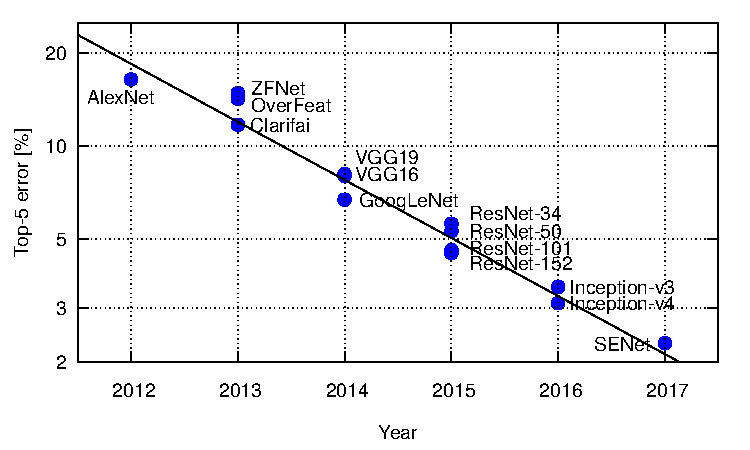
\includegraphics[width=\linewidth]{fig/y_o2.pdf}
\end{center}
\caption{Yearly error transition for ImageNet.}
\vspace*{-3pt}
%{\hfill\footnotesize Note how the caption is centered in the column.\hfill}
\end{minipage}
\begin{minipage}{0.49\hsize}
\begin{center}
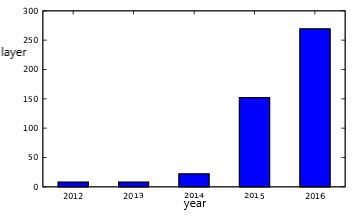
\includegraphics[width=\linewidth]{fig/fig2.png}
\end{center}
\caption{A scale change according to the year of ILSVRC championship model}
\vspace*{-3pt}
        %{\hfill\footnotesize Note how the caption is centered in the column.\hfill}
        \end{minipage}
\end{figure}


The composition of this paper is as follows. Section 2 explains the concepts of machine learning and deep learning, and the basics of neural networks and SVM used in this research.
Next, Section 3 explains the training data reduction method using support vectors, and verifies the effects of support vectors in neural network learning visually by performing preliminary experiments on multiple two-dimensional data. Section 4 shows the results of evaluation experiments using the latest neural network ResNet and the image data set CIFAR-10 and discusses the issues. Section 5 concludes with the conclusions.



\section{Related research}
This chapter describes machine learning and support vector machines as related research required to understand the proposed method. First, we will explain the components and basic principles of a neural network, which is a network model mainly used in machine learning, and then the mechanism of deep learning, which is one of machine learning methods. Next, we will describe SVM. Finally, we will talk about the existing training data reduction method.

\subsection{Machine learning}
Machine learning is a method that enables machines to learn themselves and analyze the regularity and the rule of data, instead of human beings writing all actions in the program in advance. This method makes it possible to perform specific actions by repeatedly learning and training. As an example, consider identifying images of horses and zebras. In order to identify a given image as a horse or a zebra, the machine reads a large number of images of the horse and the zebra and repeats learning. At this time, by giving instructions to pay attention to the presence or absence of the stripe pattern of the body and learning, when reading a new image of a horse or a zebra, they will be noticed and identified. As described above, it is called supervised learning that learning is performed by reading data for which answers are known in advance, which is one of the mainstream machine learning methods. Conversely, there is also unsupervised learning, but we will omit it because it is not relevant to this research.

\subsection{Neural Network}
A Neural network is a network created by mimicking the structure of the human brain. As shown in Fig. 3, it consists of nodes and synapses. Nodes are called artificial neurons, which are mathematical models created by imitating neurons in the human brain and can perform arbitrary operations. Nodes can pass computation results by connecting them, and it is the synapse used for this connection.
\begin{figure}[t]
\begin{center}
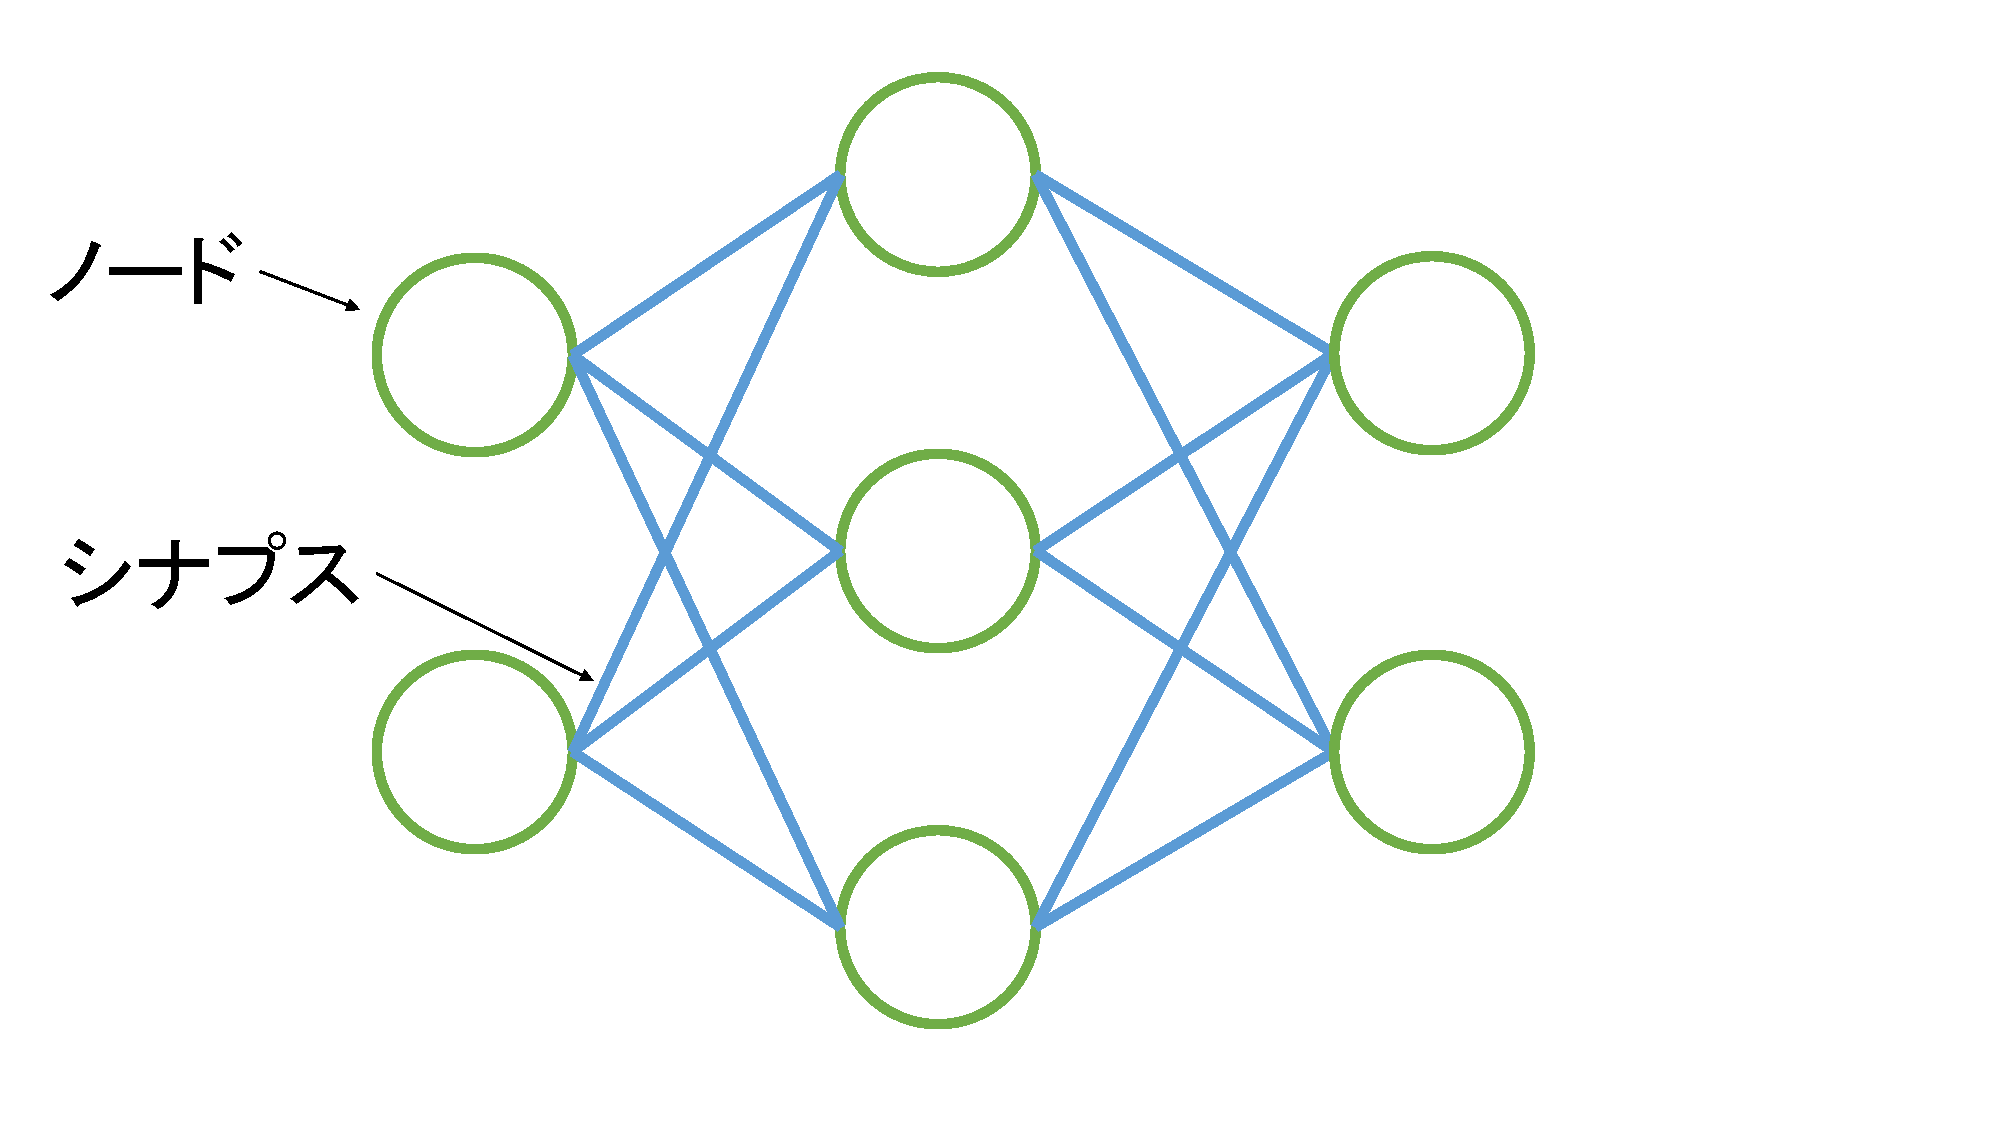
\includegraphics[width=0.6\linewidth]{fig/nn.pdf}
\end{center}
\caption{Structure of neural network.}
\vspace*{-3pt}
%{\hfill\footnotesize Note how the caption is centered in the column.\hfill}
\end{figure}


 To illustrate that neural networks can mimic the human brain's thinking circuit, as an example, we consider the question "Do you go shopping on the weekend." It is assumed that there are the following three factors as to whether to go shopping.
\begin{figure}[t]
\begin{center}
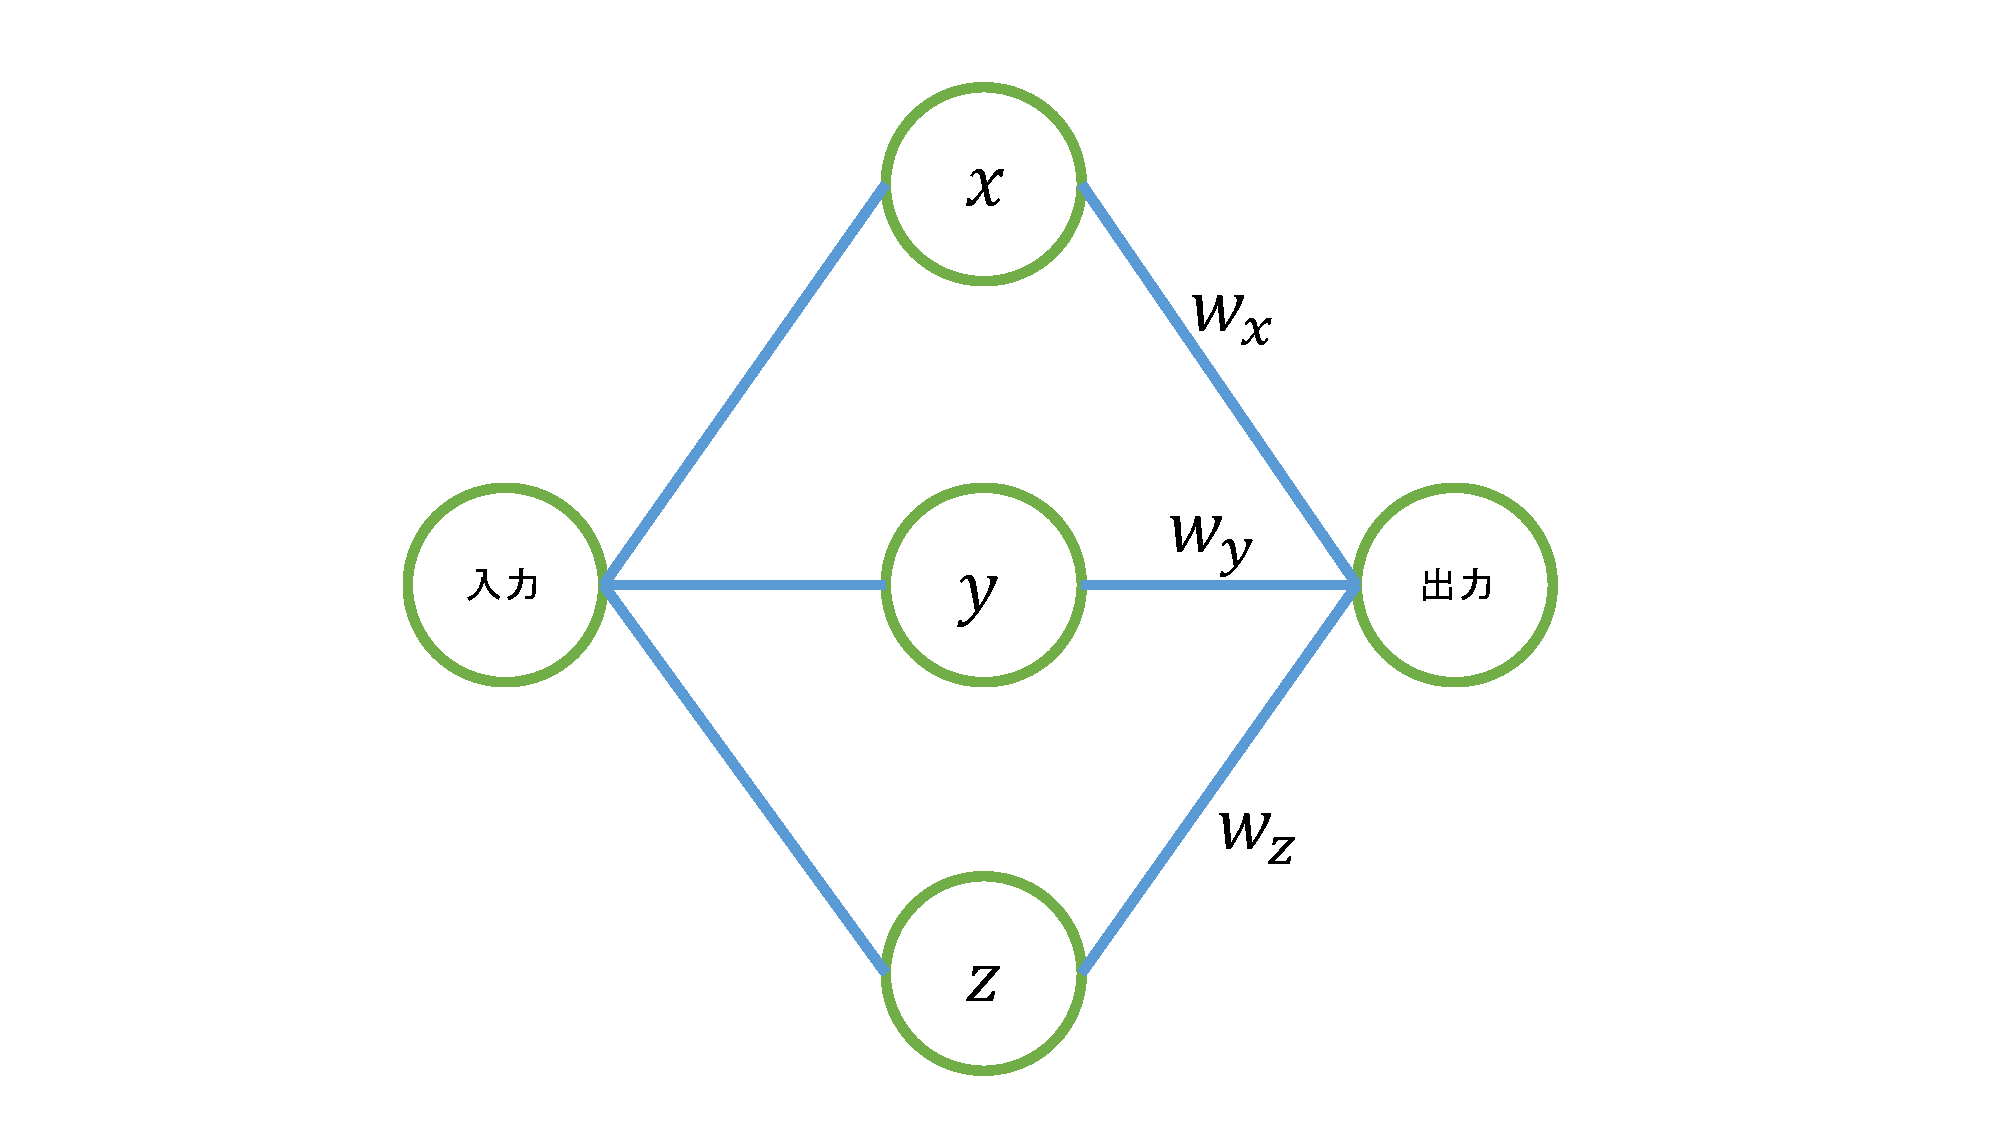
\includegraphics[width=0.8\linewidth]{fig/shopmodel.pdf}
\end{center}
\caption{Model to decide whether to go shopping.}
\vspace*{-3pt}
%{\hfill\footnotesize Note how the caption is centered in the column.\hfill}
\end{figure}
\begin{enumerate}
\item x: Closeness from home
\item y: Weather
\item z: With or without discount sale
\end{enumerate}
These outputs can be expressed as 0 or 1. For example, the output of x is one if the store is near the house, and 0 if it is far. The other two are the same. It should be noted that each factor is not an equivalent value. For example, no matter how close the store is from the house, you may never go if the weather is terrible, or even if no matter how far the store is from the house and bad the weather is, you may go if the store is making a discount sale. Such the importance of a factor is called a weight. Here, assuming that the weights of x, y and z are $w_x = 2$, $w_y = 4$ and $w_z = 8$, respectively, Fig. 4 shows a model that determines whether to go shopping. At this time, an expression indicating whether to go shopping is defined as 
\begin{equation}
xw_x+yw_y+zw_z > 5
\end{equation}
The number 5 is called the threshold, and the criterion can be changed by changing the threshold. If the threshold is 5, the shop will go shopping if it is near the house and the weather is good and if the shop is making a discount sale. In other words, if the store is near the house and the weather is good, it will go even if the store does not have a discount sale, and if it has a discount sale, other factors will be ignored. Next, assuming that the threshold is 10 and 
\begin{equation}
xw_x+yw_y+zw_z > 10
\end{equation}
if the weather is good and the store is making a discount sale, you will go shopping, and whether the store is near the house does not affect on the result. In this way, the threshold changes the criteria for deciding whether to go shopping. Although a simple network is considered in this example, if nodes are increased and more complex networks are used, more advanced judgment can be made.
 

\subsection{Deep Learning}
Deep learning is one of the machine learning methods using Deep Neural Networks (DNN). The difference between DNN and conventional neural networks is that the layers are deeply overlapped. Whereas ordinary neural networks have only one middle layer, DNN has two or more middle layers, which is a feature of DNN. Compared to ordinary neural networks, learning data, learning time, and power consumption are more massive, so that learning can be performed with higher accuracy. 
\begin{figure}[t]
\begin{center}
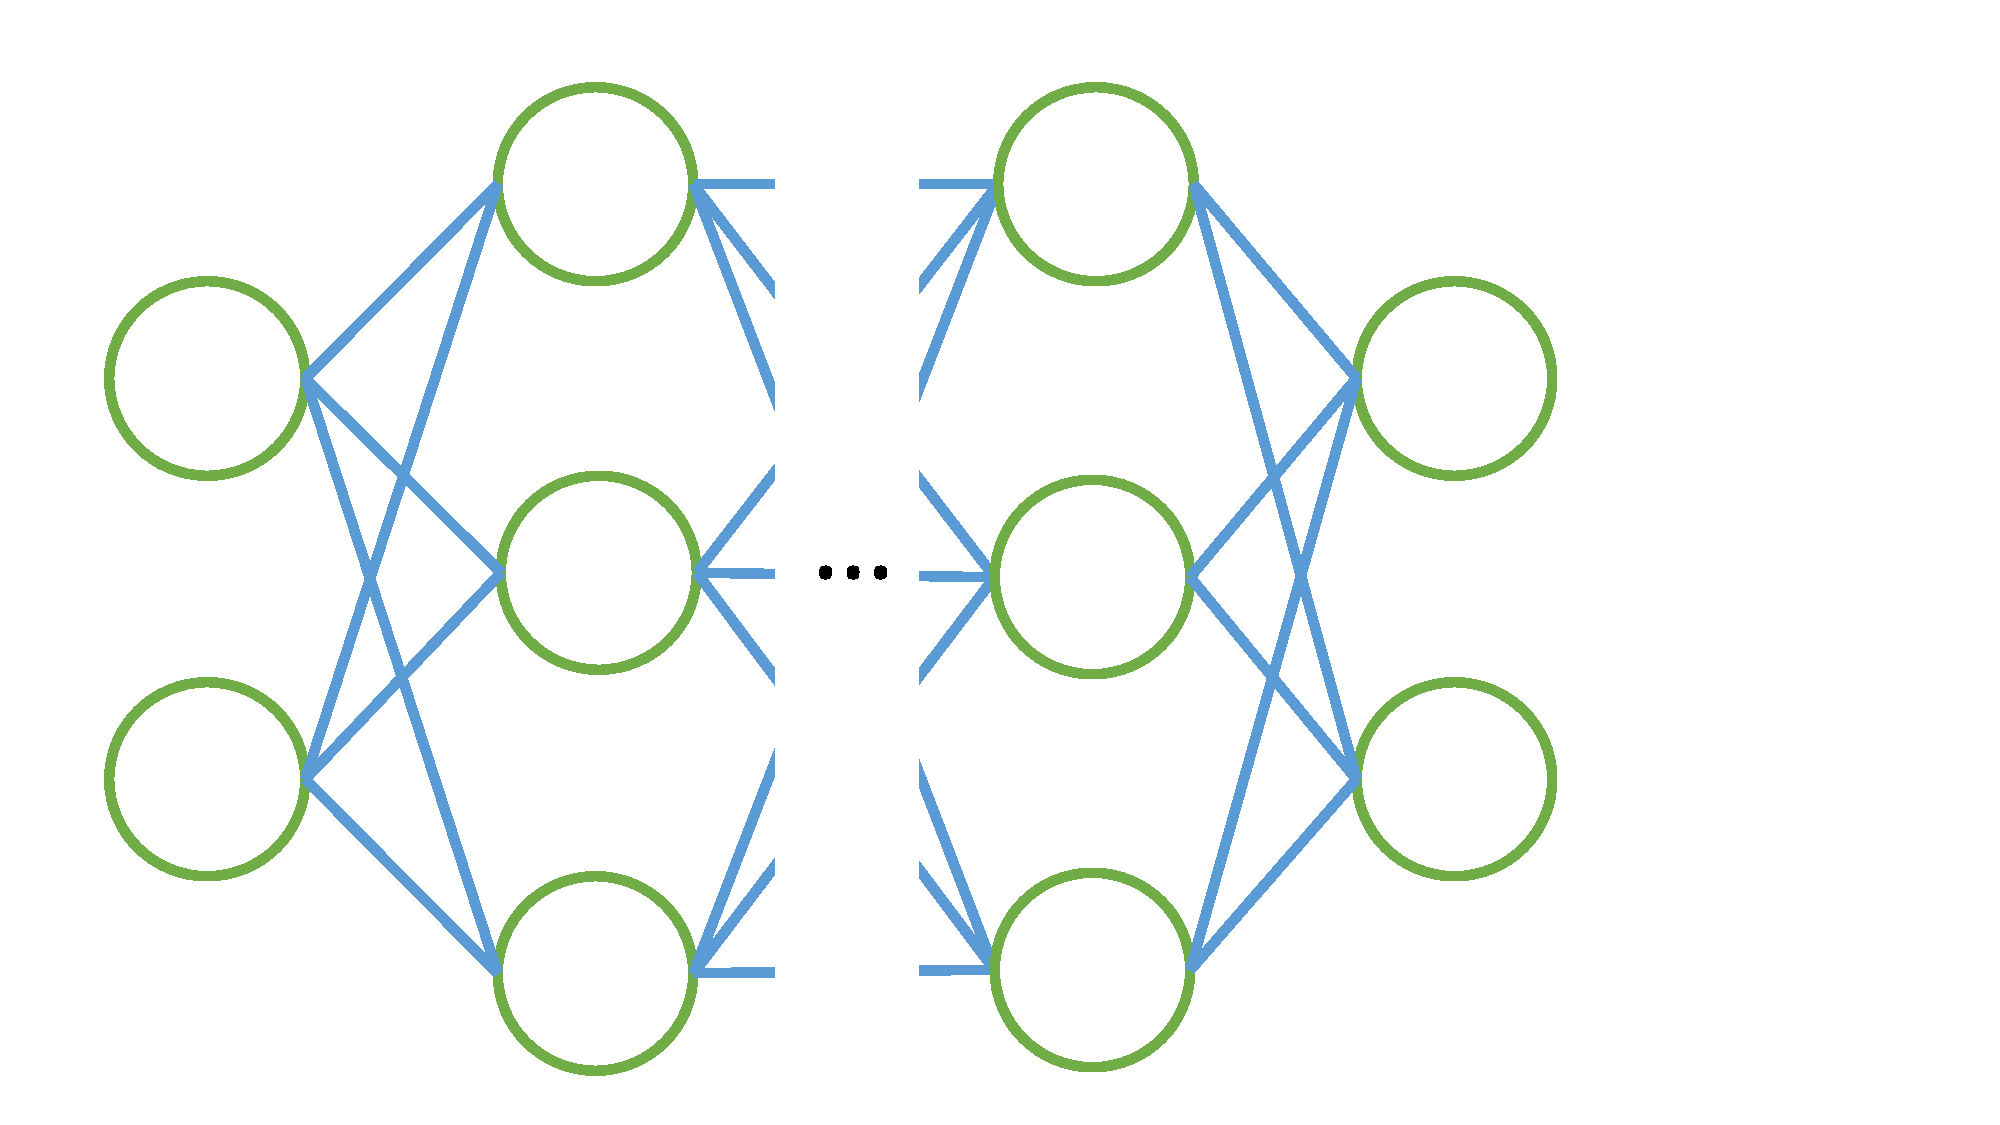
\includegraphics[width=0.6\linewidth]{fig/dnn.pdf}
\end{center}
\caption{Structure of Deep Neural Network.}
\vspace*{-3pt}
%{\hfill\footnotesize Note how the caption is centered in the column.\hfill}
\end{figure}
Usually, in machine learning, it is necessary to set in advance a factor called a feature that is an index of discrimination. However, in deep learning, features can be extracted automatically by updating the equation of nonlinear transformation performed in each layer. Here, as an example, Fig. 6 shows the results of identifying the spiral model. The figure represents that the orange background is positive, blue is negative, and white is 0, and the point is the data at that coordinate. From the input on the left side, it is understood that the division of the space is performed with a complicated curve each time the layer is advanced, and it is finally expressed as a spiral model.
\begin{figure}[t]
\begin{center}
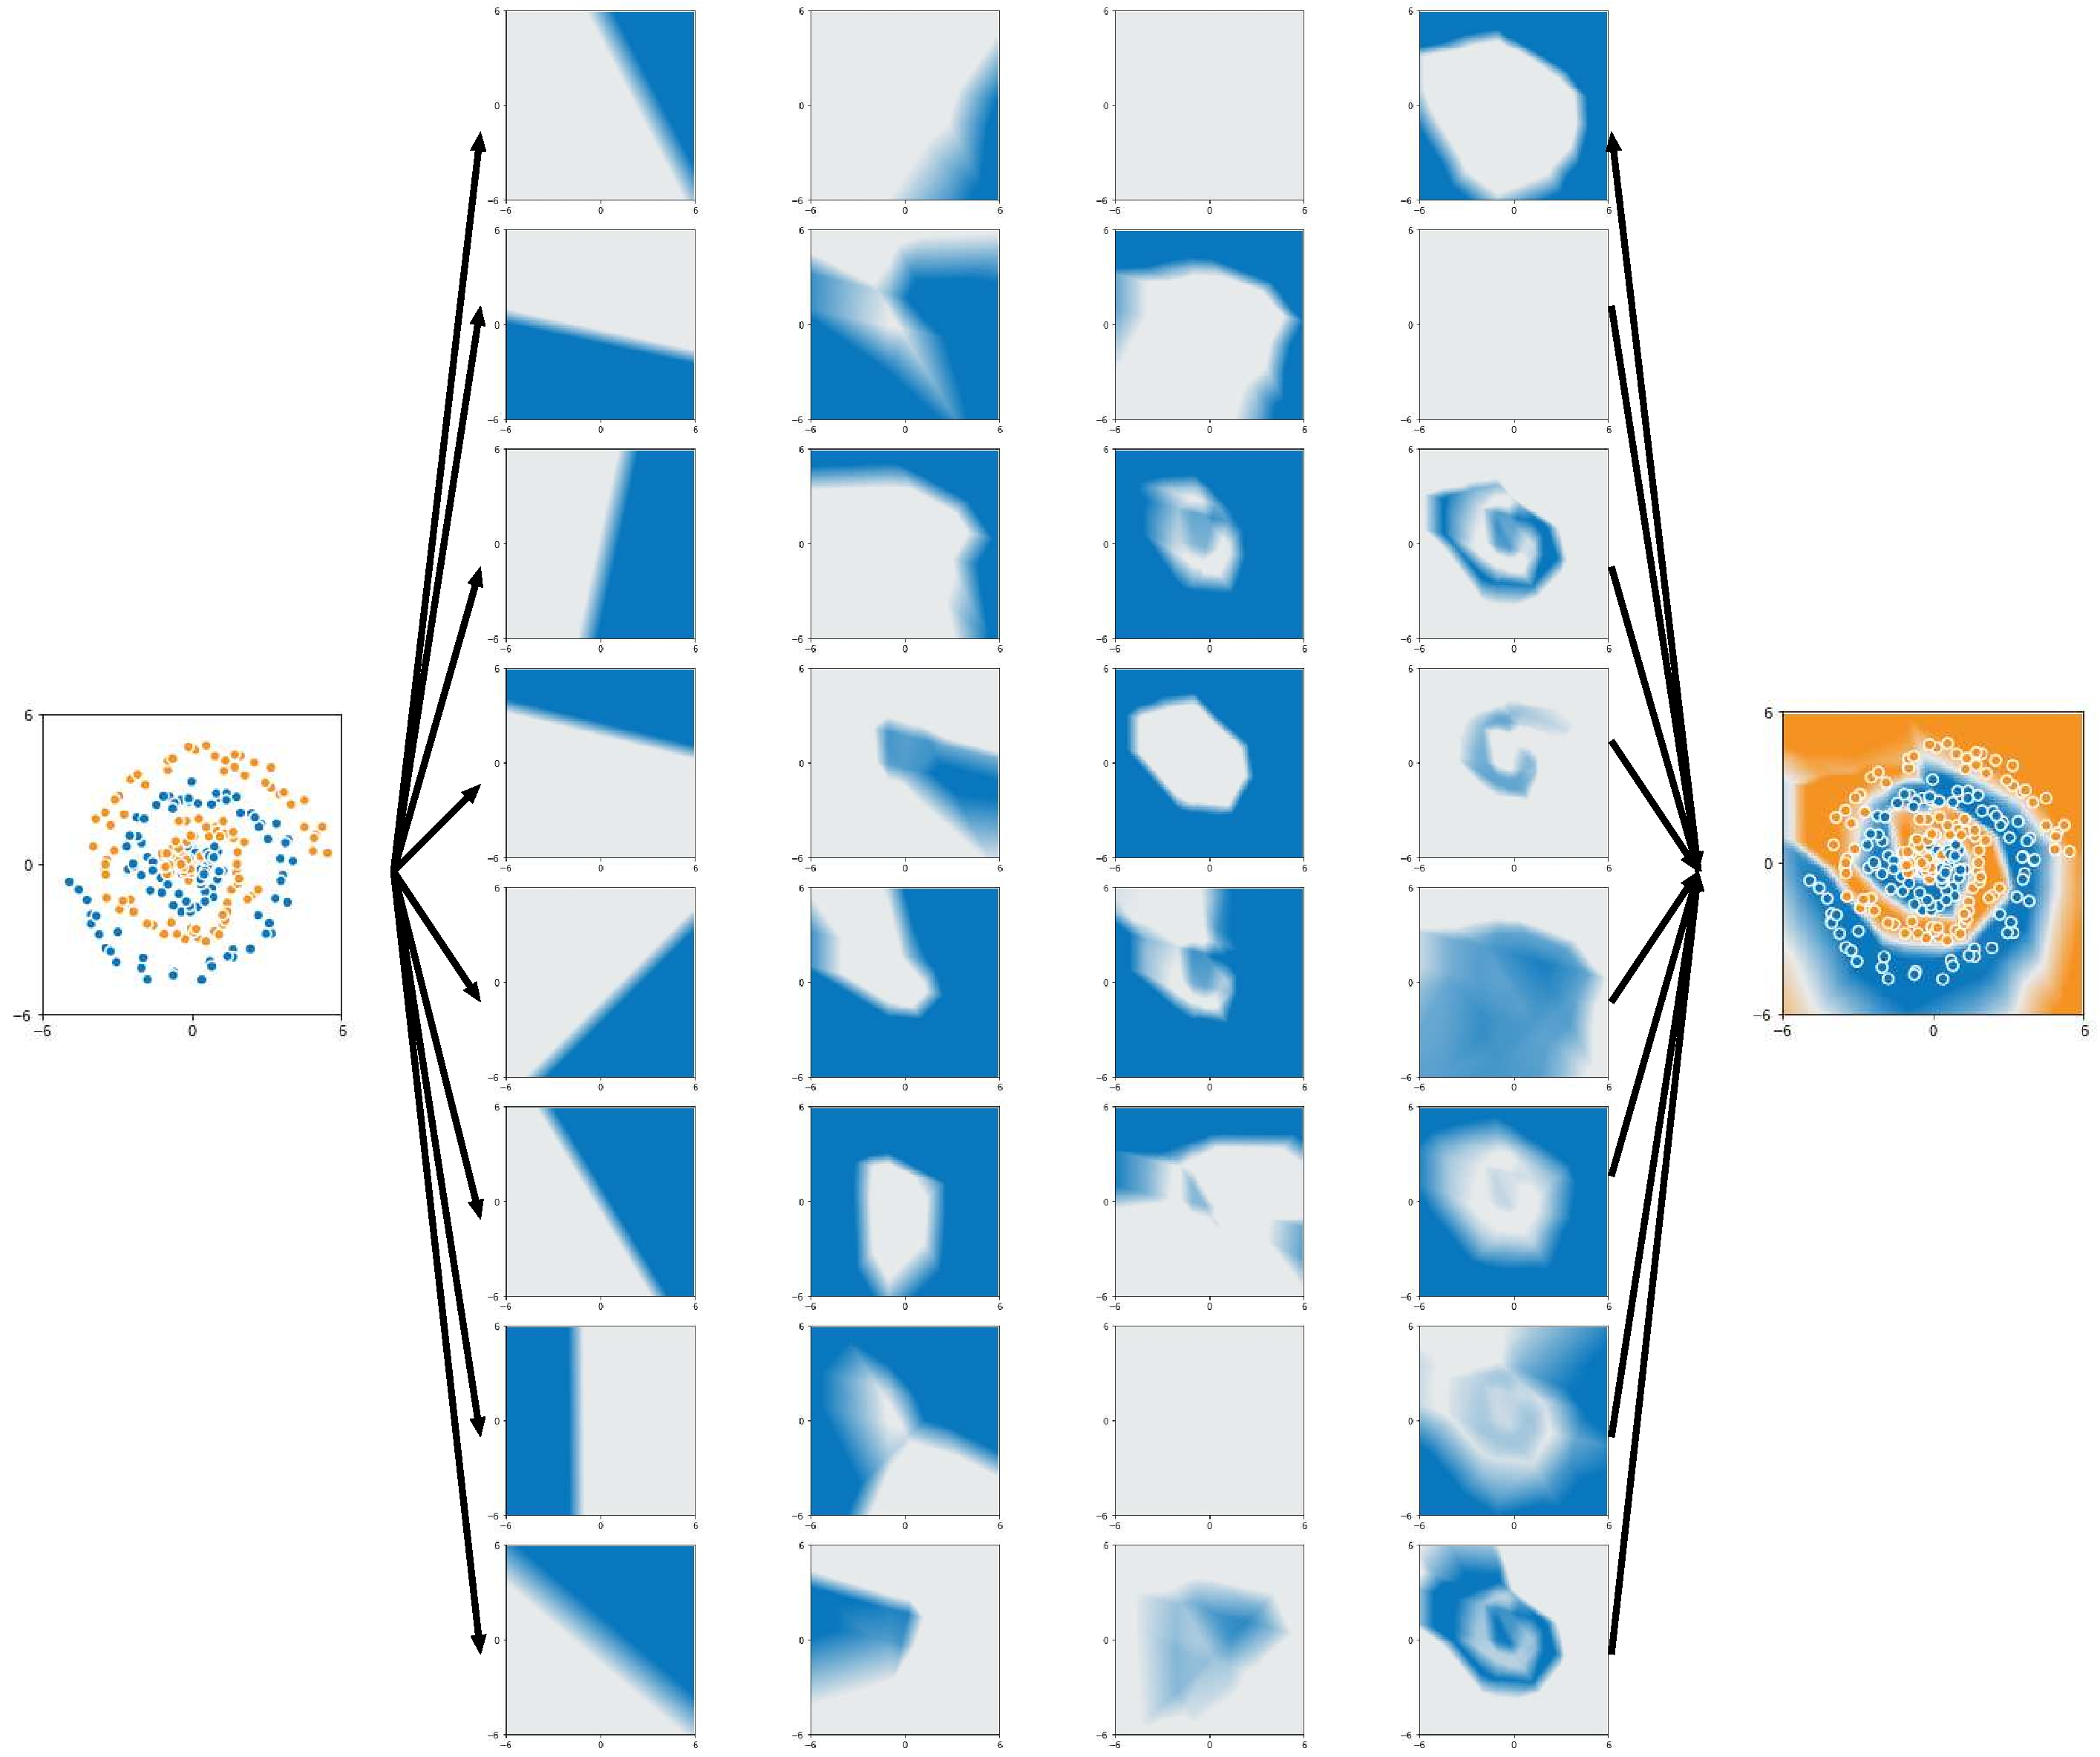
\includegraphics[width=0.8\linewidth]{fig/C_SPIRAL_ReLU_L4xN8_overall.pdf}
\end{center}
\caption{General flow of feature detection.}
\vspace*{-3pt}
%{\hfill\footnotesize Note how the caption is centered in the column.\hfill}
\end{figure}
When analyzing data such as images and sounds in deep learning, the data contains many features. In order to extract this feature without loss, it is ideal for dividing it into each, but it is very defficult because the features are not always arranged at equal intervals and we do not even know what the features are at first. Therefore, it is essential to divide data without loss of features as much as possible. Here, image identification is considered as an example. If the criterion for determining whether it is kangaroo is the presence or absence of a pouch, the judgment can not be made if the portion of the pouch is on the boundary of the data division and divided into two. Thus, depending on the method of data division, features may be lost. In order to solve this, we use an overlapping method. This is a method of dividing the data by overlapping them to some extent. If it explains in the character string "abcde" for the sake of simplicity, this method is not divided into "abc" and "de" but divided into "abc", "bcd" and "cde." This can reduce the loss of features, which contributes to the increase in data analysis accuracy. 

When the data is divided and passed to each node in the first layer, the processing is performed for each node, and the data is propagated to the nodes in the next layer. At this time, each node is still in the condition that it has features required and unnecessary features(errors) to produce accurate results. If all the information is passed to the next layer, all the errors will be transmitted, and if the information passed is too small to pass the errors, the features will be lost. Here, the calculation formula applied when passing data to the next layer is called the activation function. The activation function can convey features to the next layer more clearly by slightly changing the original data, and has the effect of suppressing overfitting. There are several types of activation functions, and two primary sigmoid functions and ReLU functions are described. 

The sigmoid function is shown in Fig. 7 is a function that approaches one as the value of the input increases and approaches 0 as it decreases. The characteristic is that it is a monotonically increasing function, and it does not become one regardless of how big the original input is, and does not become -1 regardless of how small it is. The sigmoid function is shown in (3).
\begin{figure}[t]
\begin{center}
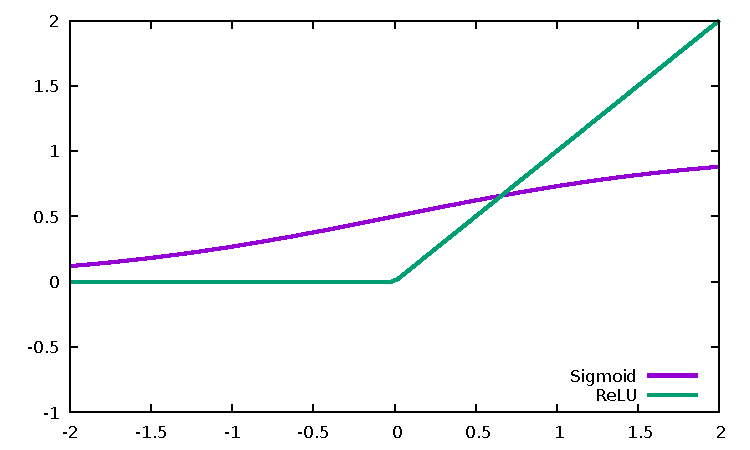
\includegraphics[width=0.8\linewidth]{fig/act.pdf}
\end{center}
\caption{Activation function.}
\vspace*{-3pt}
%{\hfill\footnotesize Note how the caption is centered in the column.\hfill}
\end{figure}
\begin{equation}
h_{sigmoid}(x)=\frac{1}{1+e^{-x}}
\end{equation}
The sigmoid function can maintain the original input characteristics to some extent but has the disadvantage that the computational complexity increases. The characteristic is that the change in value becomes gentler as it gets closer to -1 and 1, and the gradient when differentiating the sigmoid function is 
\begin{equation}
h'_{sigmoid}(x)=(1-h_{sigmoid}(x))h_{sigmoid}(x)
\end{equation}
and is almost 0 in the vicinity of those values. In other words, features tend to be flat at these values, and as the layer gets deeper, features tend to be lost, and learning may not progress. Therefore, along with the problem of computational complexity, it is often used in ordinary neural networks with few layers, but it is not often used in DNN.

In light of the shortcomings of sigmoid functions, DNN often uses the ReLU (Rectified Linear Unit) function shown in Fig. 7. The ReLU function is a function that outputs 0 when the input is 0 or less and outputs the input value as it is when 0 or more. The process is simpler than the sigmoid function, and the equation is as follows.
\begin{equation}
h_{ReLU}(x)=max(0,x)
\end{equation}
Because the ReLU function is linear, differentiation does not result in a zero gradient. As a result, there is no problem that learning will not progress due to the loss of features, which has been an issue with sigmoid functions. The calculation is also straightforward, and DNN often uses the ReLU function.

\subsection{Support Vector Machine}
Support Vector Machine (SVM) ~\cite{bib:Support-Vector-Networks} is one of pattern recognition models using supervised learning and is a method that can be used for classification and regression problems. In describing the concept of SVM, consider the problem of classifying the distribution map, as shown in Fig. 8(a). This figure is a graph representing the distribution with x as the horizontal axis and y as the vertical axis. We consider classifying orange and blue data into one hyperplane. There are many division methods, but arbitrary division methods are not possible. As an example, Fig. 8(b) shows two ways of drawing below. The two divisions are shown in Fig. 8(b) can not be regarded as incorrect because both can correctly classify orange and blue. Assuming that both lines are suitable for classification, we consider the input data shown in black. Because these input data belong to the orange side in one line and to the blue side in the other line, these lines are not suitable for classification. In this way, the data near the boundaries to be classified are vague data. SVM is a method to classify this ambiguous data as correctly as possible.
\begin{figure}[t]
  \begin{center}
    \subfigure[training data]{
      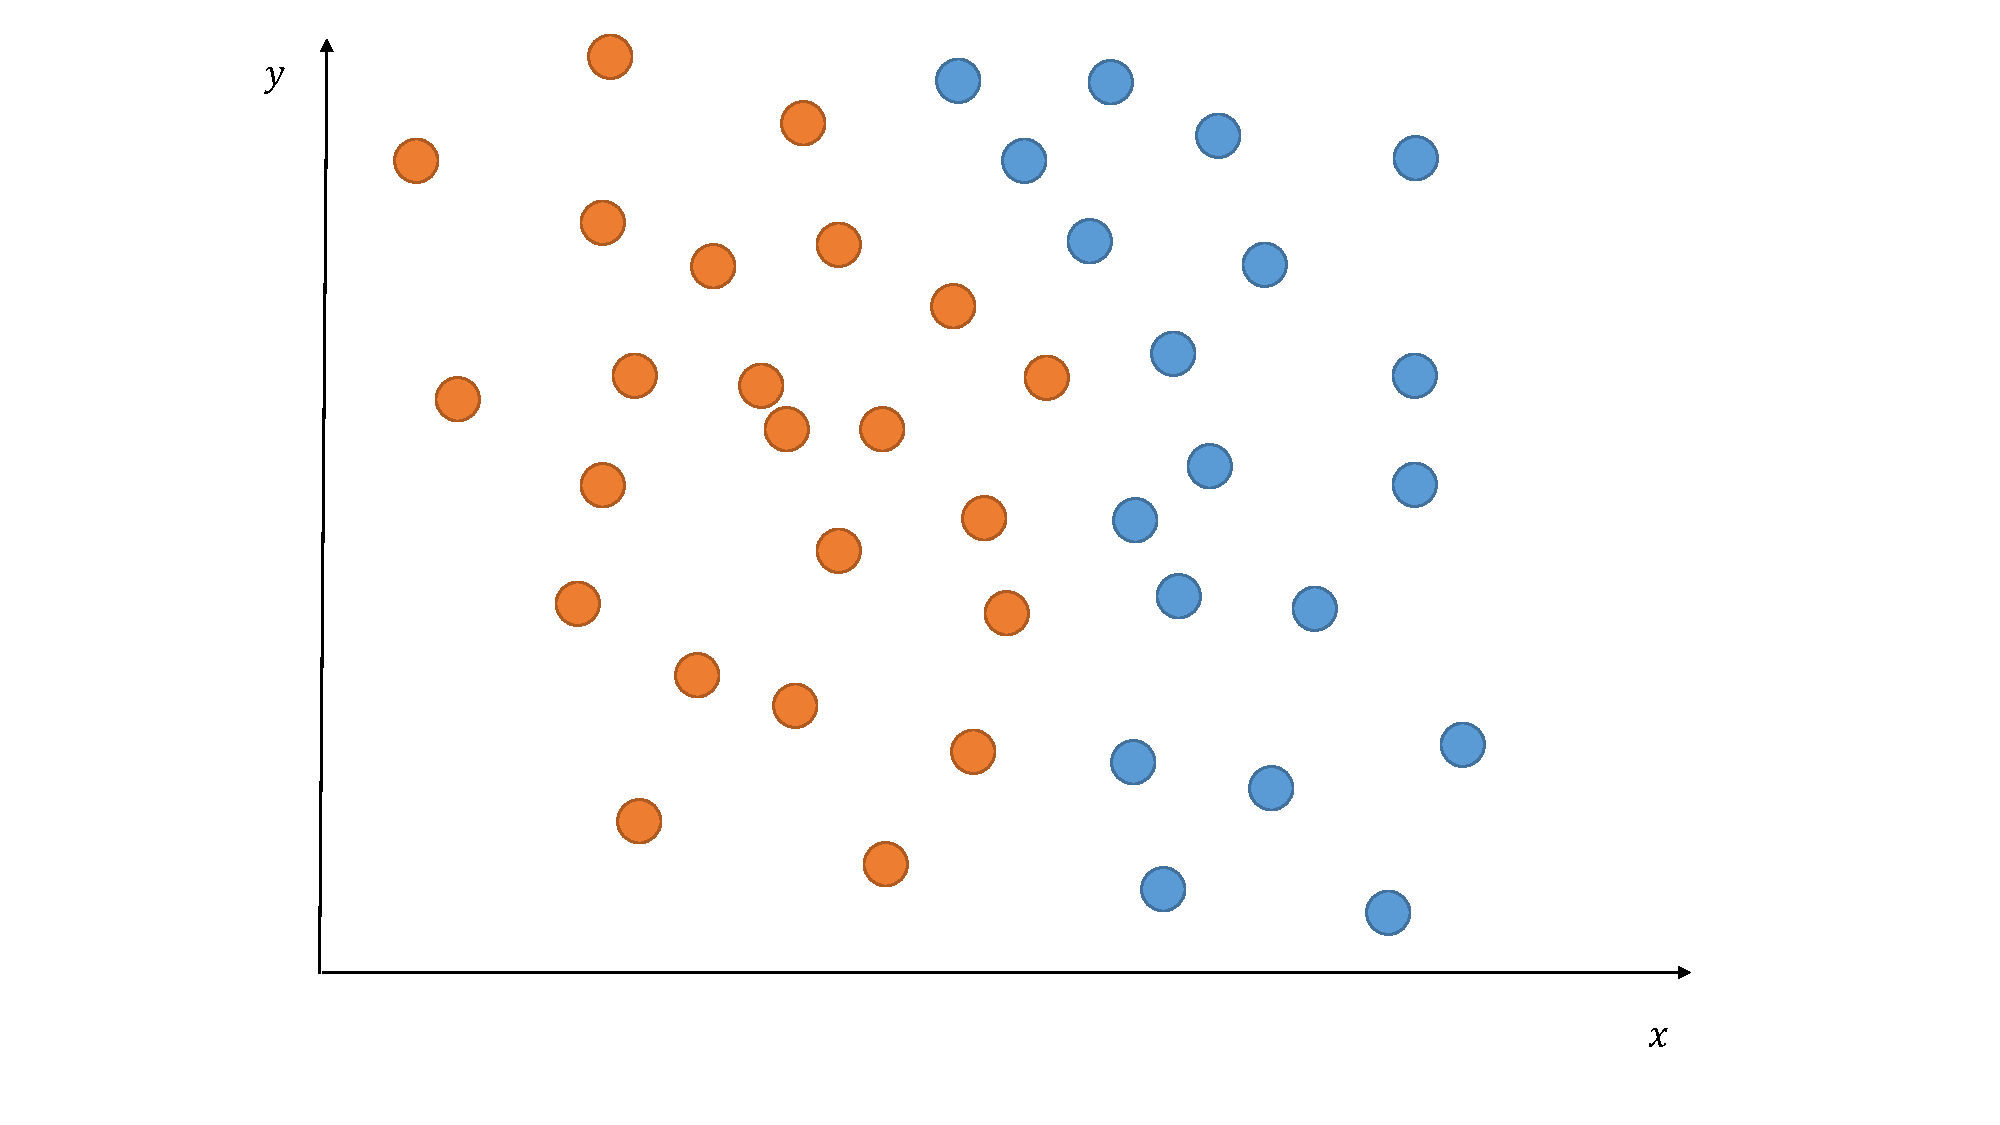
\includegraphics[width=0.48\linewidth]{fig/dist.pdf}}
      \subfigure[Classification result by difference of discrimination hyperplane.]{
      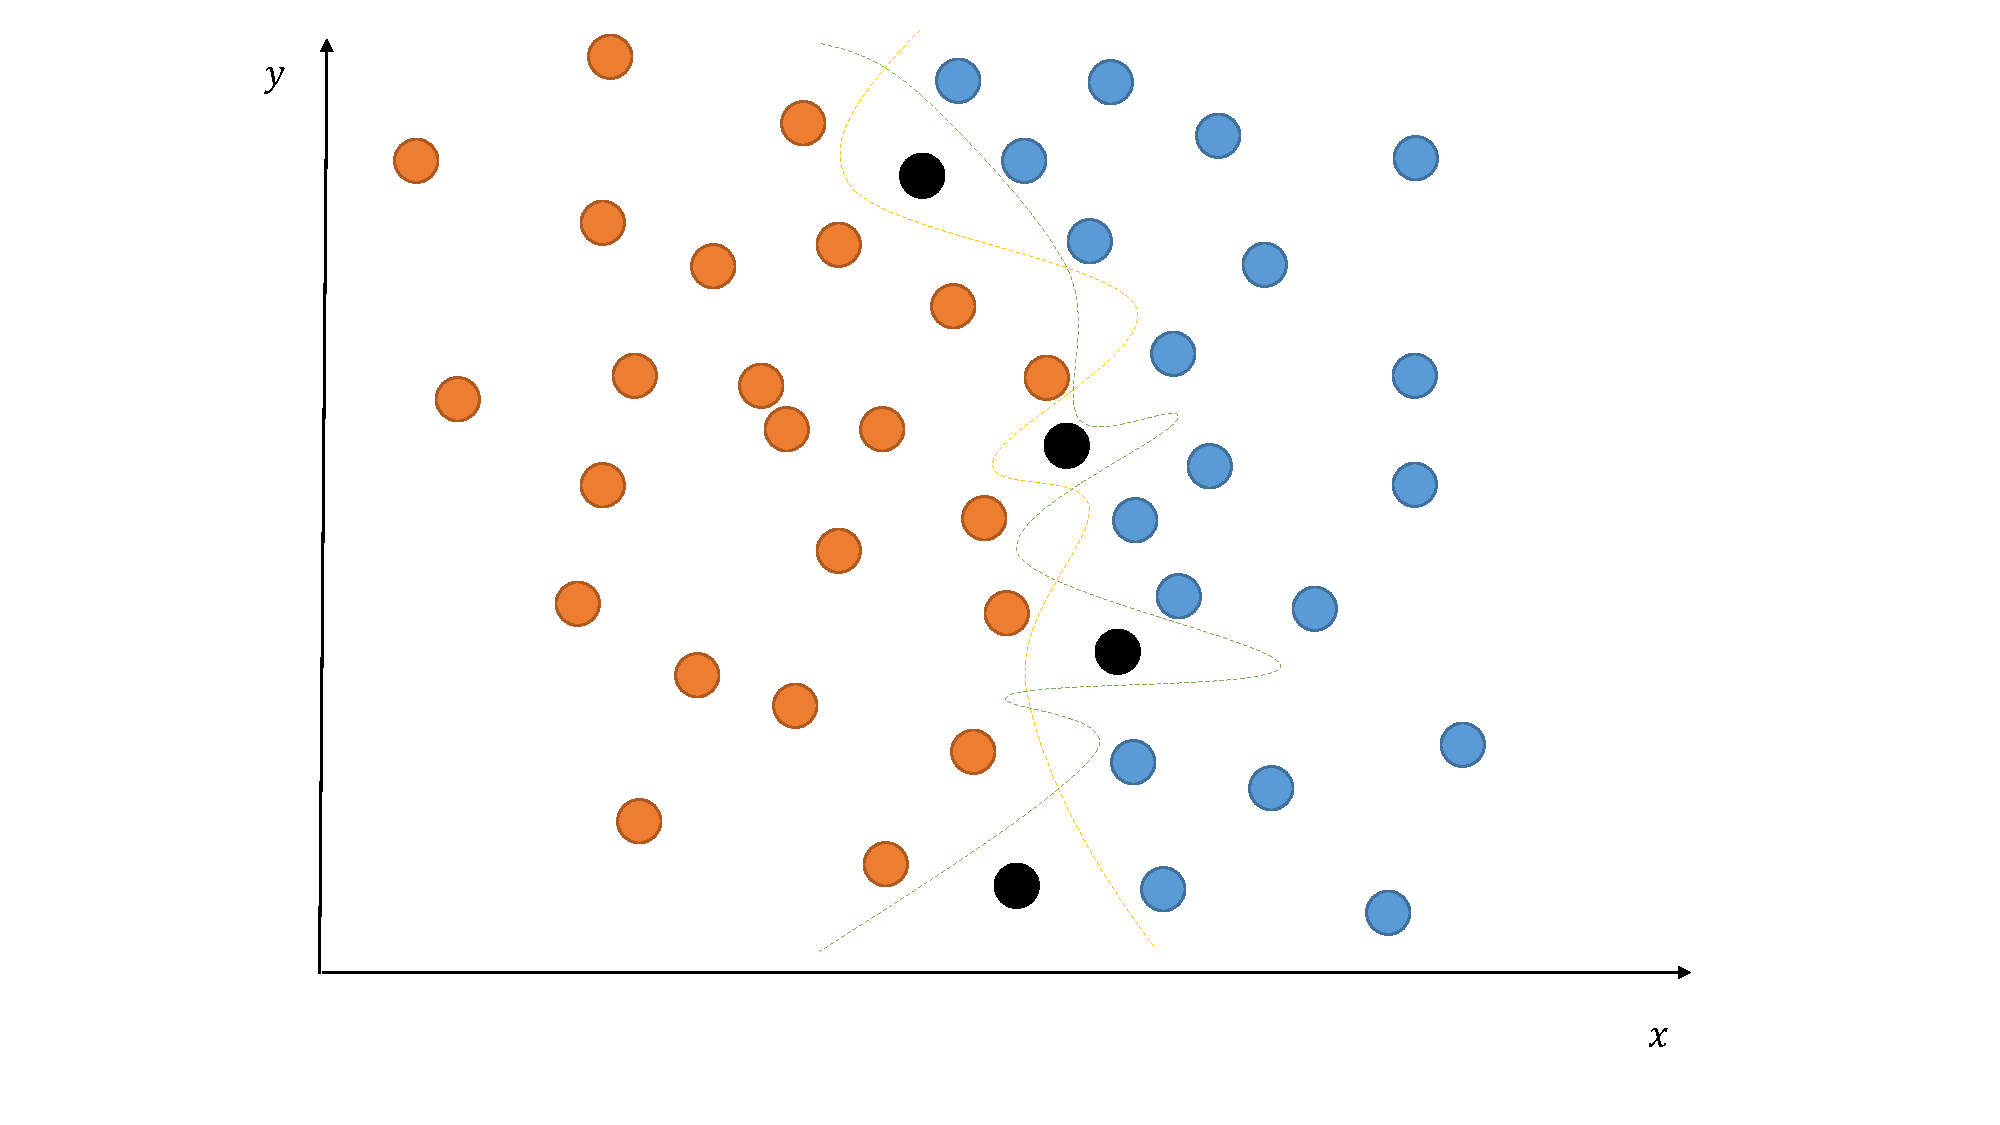
\includegraphics[width=0.48\linewidth]{fig/dist_line.pdf}}
\end{center}
\caption{Example of different classification for the same data.}
\vspace*{-3pt}
%{\hfill\footnotesize Note how the caption is centered in the column.\hfill}
\end{figure}
SVM components have support vectors and margins. The support vector is the data near the classified boundary, and the margin is the distance between the classified boundary and the data. The above vague data is data that is close to the boundary; in other words, data with a small margin. If there are many data with a small margin, the classification accuracy will be reduced, and such data can be reduced by making the margin as large as possible. This is called margin maximization. In order to prevent incorrect classification, it is only necessary to classify the data near the boundary correctly. Therefore, classification is performed by focusing on the support vectors. This concept is used in the proposed method described later. Fig. 9 shows how support vectors reduce data.
\begin{figure}[t]
  \begin{center}
    \subfigure[training data]{
      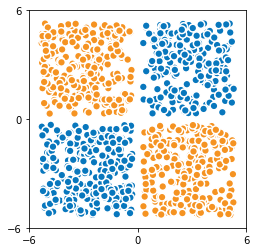
\includegraphics[width=0.35\linewidth]{data/C_XOR/inputdata2.png}}
    \subfigure[support vector]{
      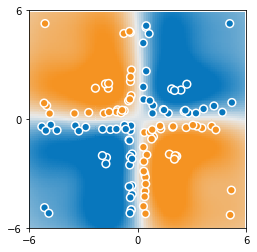
\includegraphics[width=0.35\linewidth]{data/C_XOR/SVMdata2.png}}
  \end{center}
  \caption{Data reduction by support vector for XOR.}
\vspace*{-3pt}
%{\hfill\footnotesize Note how the caption is centered in the column.\hfill}
\end{figure}

\begin{figure}[t]
\begin{center}
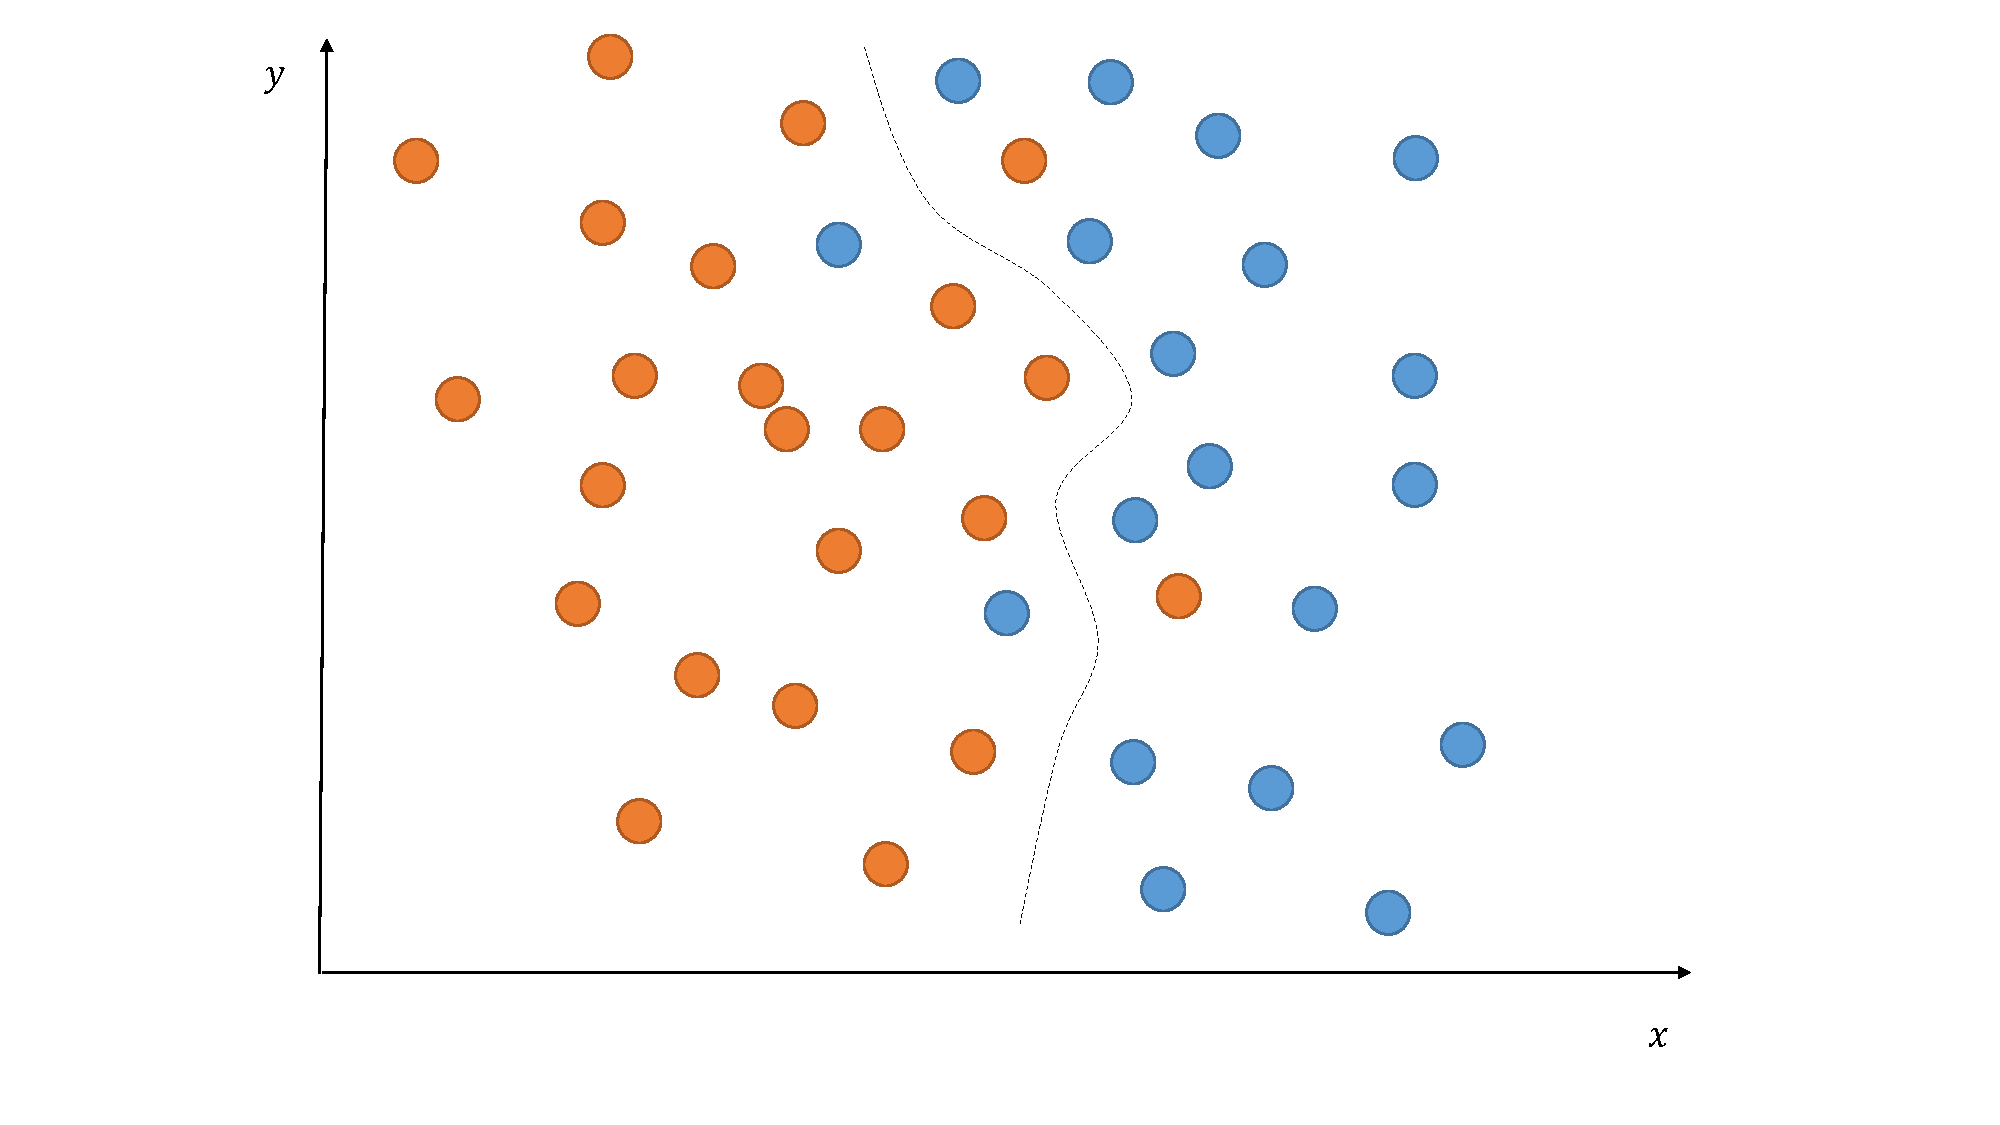
\includegraphics[width=0.8\linewidth]{fig/dist2.pdf}
\end{center}
\caption{Example of misclassification.}
\vspace*{-3pt}
%{\hfill\footnotesize Note how the caption is centered in the column.\hfill}
\end{figure}

\begin{figure}[t]
  \begin{center}
    \subfigure[Hard margin]{
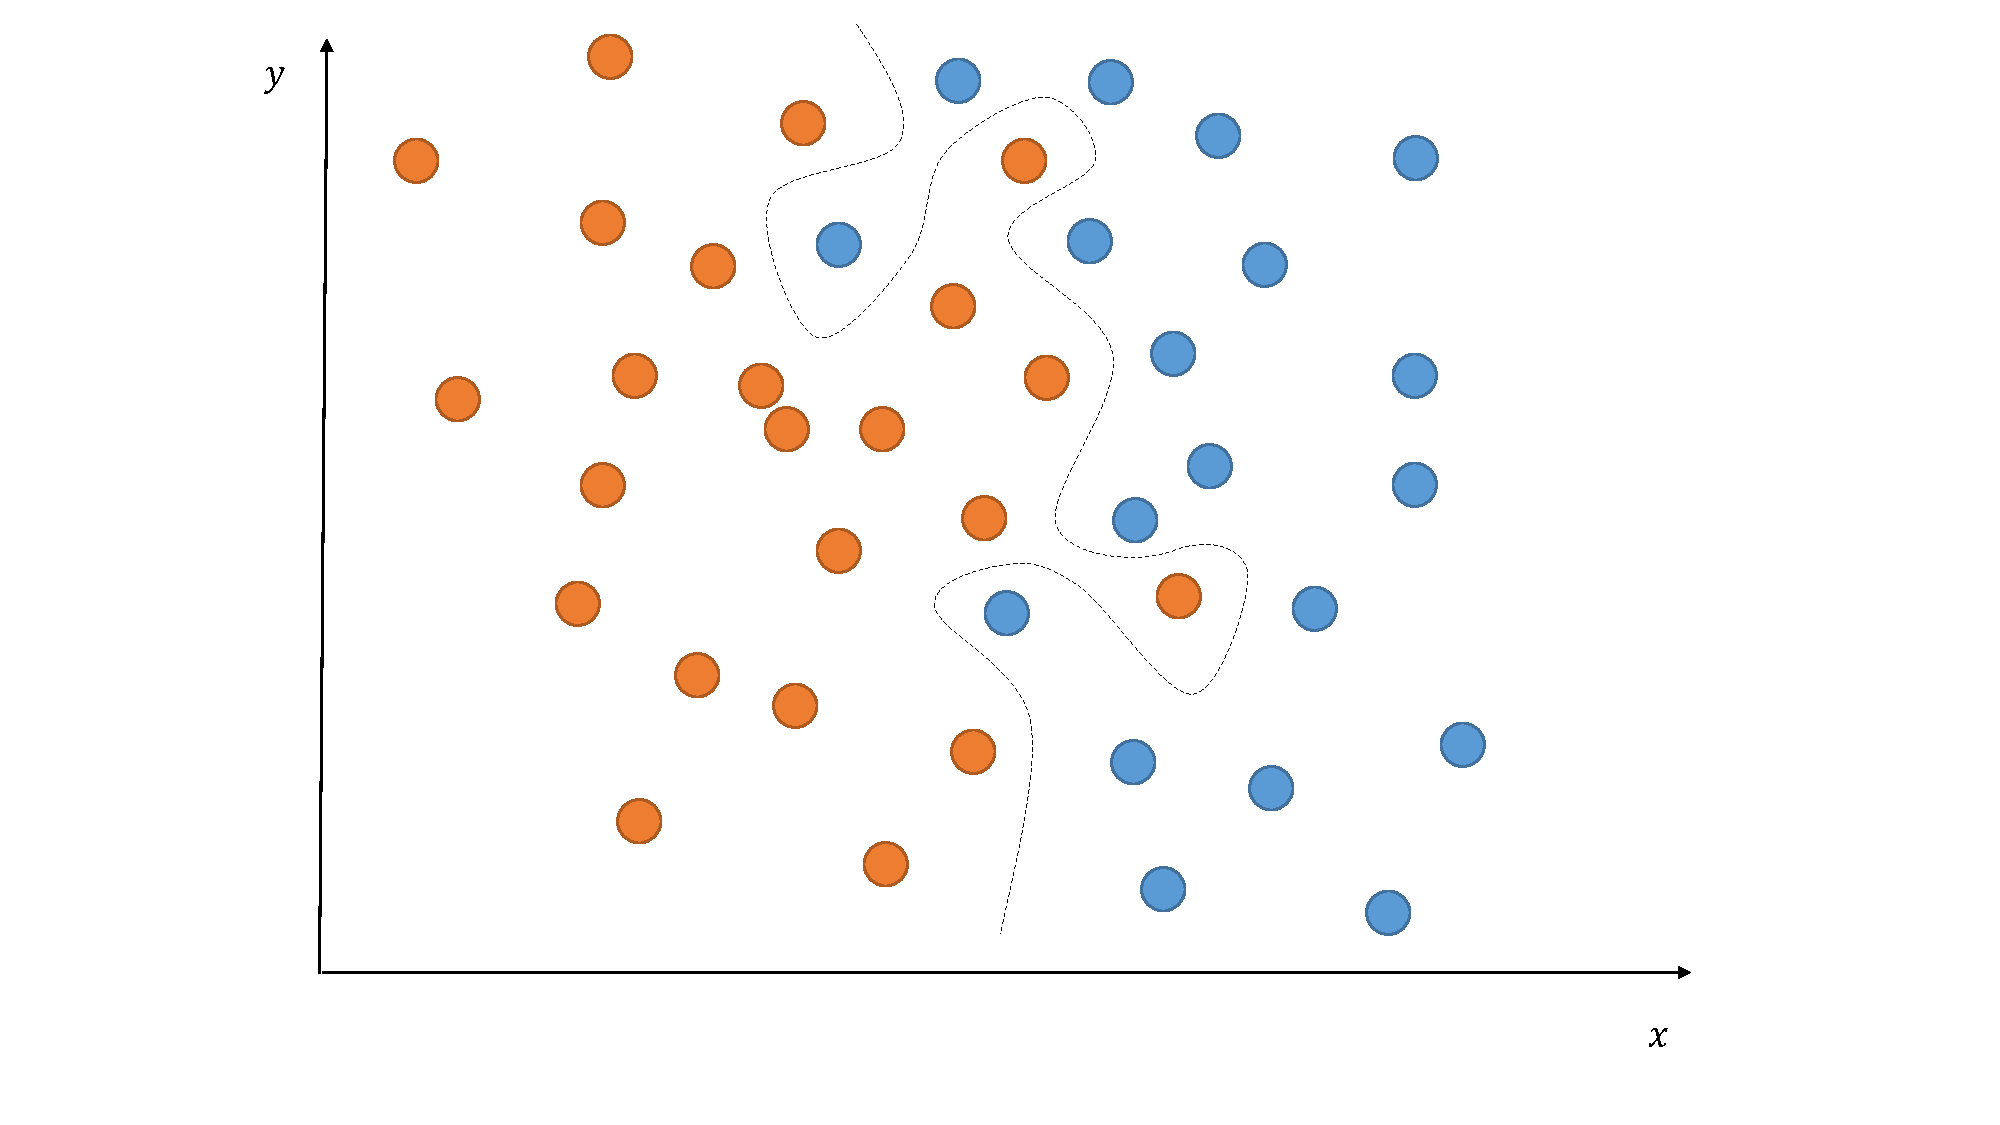
\includegraphics[width=0.45\linewidth]{fig/hardmargin.pdf}}
\subfigure[Soft margin]{
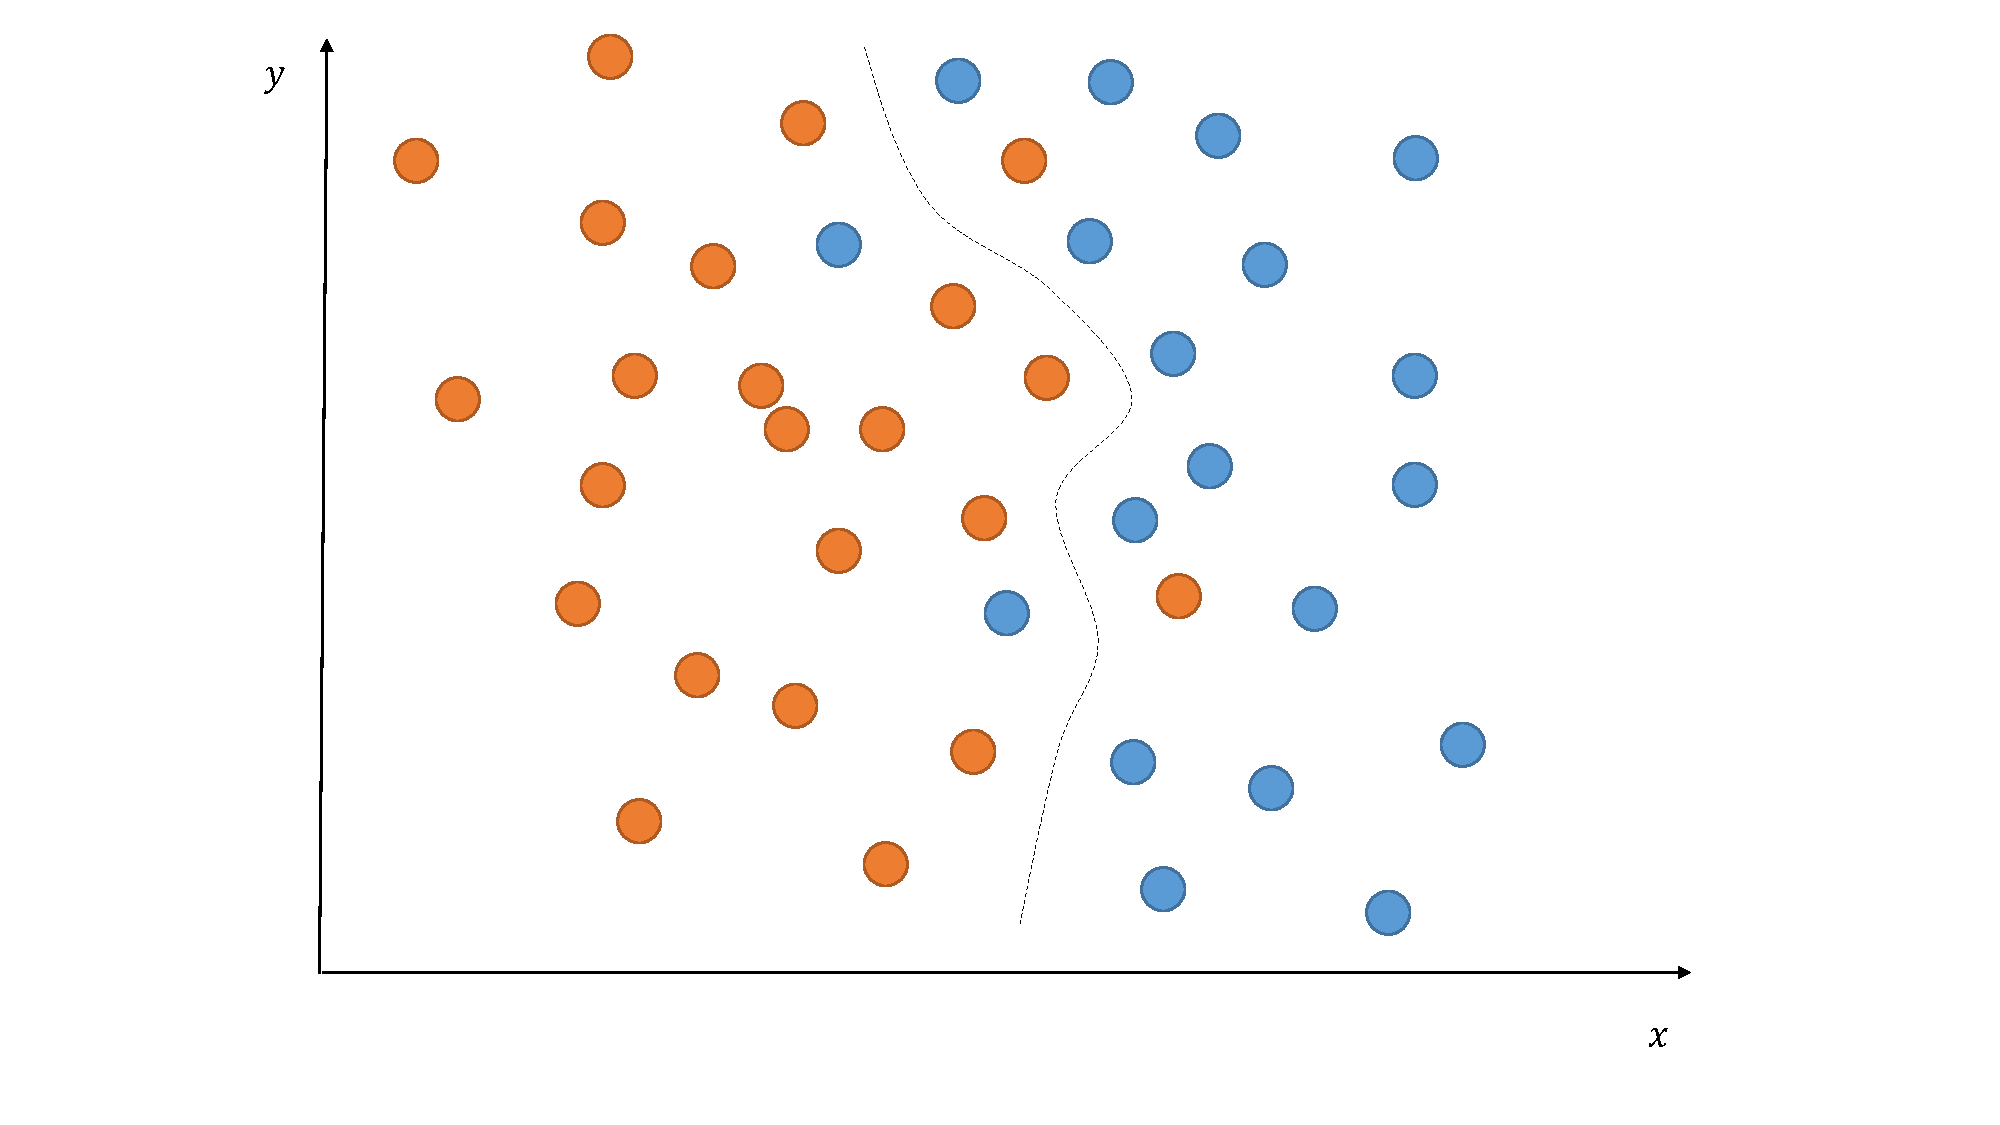
\includegraphics[width=0.45\linewidth]{fig/dist2.pdf}}
\end{center}
\caption{Hard and soft margin.}
\vspace*{-3pt}
%{\hfill\footnotesize Note how the caption is centered in the column.\hfill}
\end{figure}

Up to this point, data that can be classified finely for simplicity is taken as an example, but let us consider the case where somewhat specific data, as shown in Fig. 10, is given. If this data is classified in the same line as before, an incorrect identification will occur. Forcing correct classification of incorrectly identified data will lead to loss of these valuable data. It is called overfitting ~\cite{bib:Lessons-in-Neural-Network-Training} that it overfits the original data and the prediction accuracy for the newly given data falls. It is said that there is generalization ~\cite{bib:Generalization-in-Deep-Learning} that can be flexibly predicted for given data without causing overfitting, and tolerating an incorrect identification to some extent leads to an increase in generalization. In generalization, a technique that does not allow false identification is called a hard margin, and a technique that allows false identification to some extent is called a soft margin ~\cite{bib:An-introduction-to-kernel-based-learning-algorithms}. The soft margin allows some misidentification, but it balances the margin maximization and the allowance of the misidentification by giving a penalty. This penalty is also called cost. By adjusting the value of the cost parameter $C$, it is possible to decide how much misidentification is permitted. The following minimization problem replaces margin maximization.
\begin{equation}
\min \{\frac{1}{2}\|\beta\|^2+C\sum_{i=1}^{N}\xi_i \}
\end{equation}
$\xi$ is a slack variable, $\xi = 0$ if the data is correctly identified, $0<\xi\leq1$ if correctly identified but within the margin, and $\xi>1$ if false. That is since the second term becomes larger as there are more misidentifications, if (6) is to be minimized, an adjustment is made to reduce the value of $\xi$. It has been stated that it is possible to decide how much to allow erroneous identification by adjusting the value of the cost parameter $C$. The reason for this is the larger the value of $C$, the larger the value of the second term. Also, the case of $C \to \infty$ is called the hard margin. In the case of soft margin, adjusting the value of C can change how much incorrect identification is allowed. 

In SVM, two kernel methods, RBF (Radial Basis Function) kernel and polynomial kernel, are widely used for classification. The kernel method is a data analysis method developed from the 1990s when the proposal of SVM started, and it is a convenient method when dealing with nonlinear data. As an example, circularly distributed nonlinear data, as shown in Fig. 12(a) cannot be classified linearly.
\begin{figure}[t]
  \begin{center}
    \subfigure[Example of data that can not be classified linearly]{
      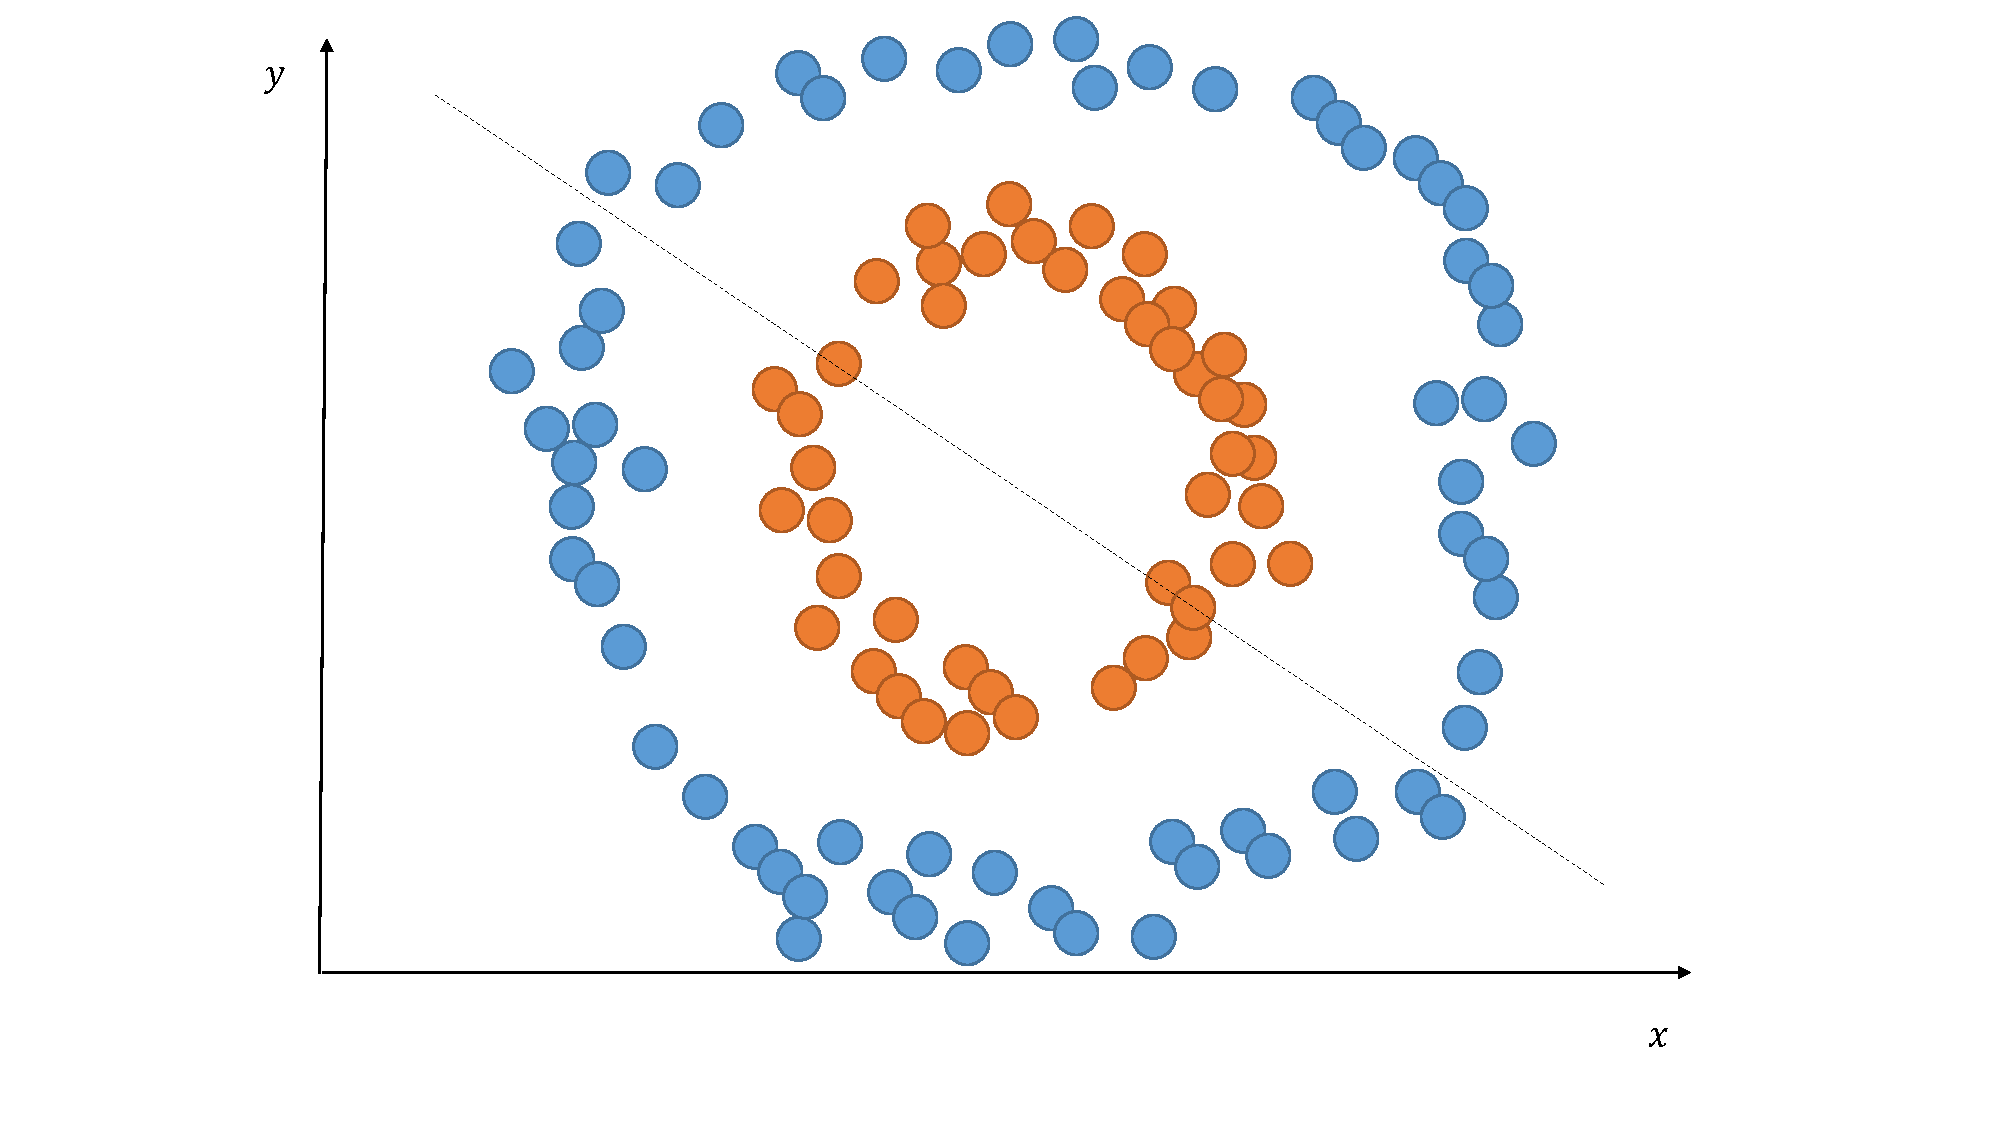
\includegraphics[width=0.48\linewidth]{fig/circle.pdf}}
    \subfigure[Convert to data that can be classified linearly]{
        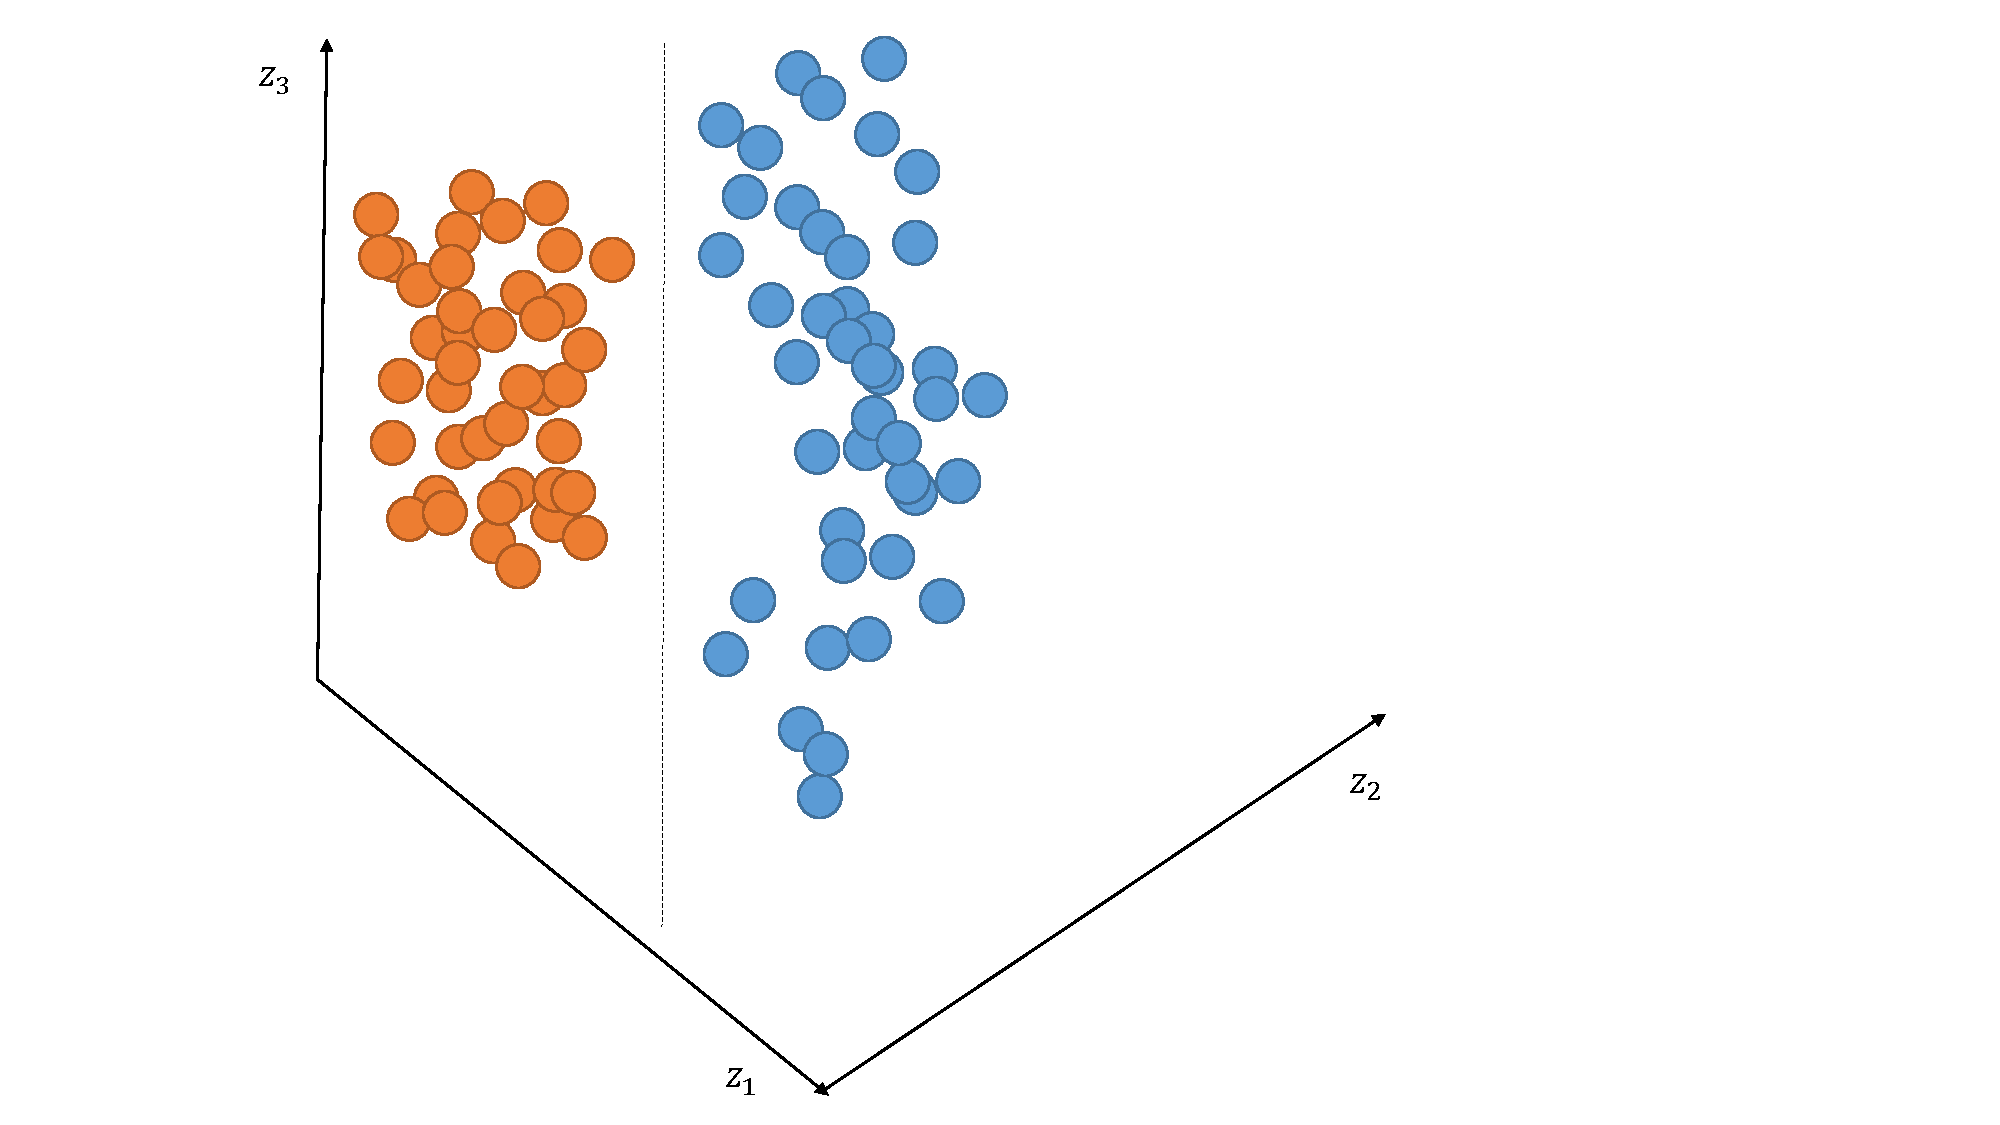
\includegraphics[width=0.48\linewidth]{fig/transcircle.pdf}}
\end{center}
\caption{Transformation of nonlinear data by kernel method.}
\vspace*{-3pt}
%{\hfill\footnotesize Note how the caption is centered in the column.\hfill}
\end{figure}
\begin{equation}
(z_1,z_2,z_3) = (x^2,y^2,\sqrt{2}xy)
\end{equation}
By using the kernel method for coordinate conversion, data that cannot be classified linearly can be converted to data that can be classified linearly. The following equation represents the RBF kernel of the two kernels used in my evaluation. 
\begin{equation}
K_p(x_i,x_j) = \exp(-\gamma\|x_i-x_j\|^2)
\end{equation}
The RBF kernel is a frequently used kernel function and often uses $C$ and $\gamma$ as hyperparameters of SVM. Next, the equation for the polynomial kernel is as follows.
\begin{equation}
K_p(x_i,x_j) = {x_ix_j+r}^{d}
\end{equation}
This is a kernel represented by a polynomial of order $d$, with $r$ added as a hyperparameter. Sections 3 and 4 show how effective these two kernel functions are for reducing training data. 

\subsection{Training data reduction method}
We consider two existing studies on training data reduction. The first is a study by Nguyen et al. using support vectors to examine how training data reduction and classification accuracy change with two-dimensional data ~\cite{bib:Support-Vector-Machines-Data-Reduction-and-Approximate-Kernel-Matrices}. This study describes the trade-off between classification accuracy when data reduction is performed using support vectors, and the problem of classifying three different data distributions: Gaussian, sine, and an ellipse, which are two-dimensional data. This derives an upper limit on how much data reduction is possible by the support vector, and it has been shown that training data can be reduced by an appropriate amount within a predetermined tolerance range. It is found that the reduction of training data by support vectors is effective in classification problems of 2D data.

 Next, as the second existing study, we describe training data reduction using support vectors for neural networks conducted by Dahiya et al. ~\cite{bib:Reducing-Neural-Network-Training-Data-using-Support-Vectors}. In this study, support vector is used to reduce training data while maintaining accuracy for the problem of classifying image dataset of handwritten numbers from 0 to 9 called MNIST shown in Fig. 13 ~\cite{bib:A-novel-hybrid-CNN-SVM-classifier-for-recognizing-handwritten-digits}. Table 1 shows the experimental results. In this research, it was reported that accuracy degradation did not occur even if the training data of 60,000 were reduced to 20,000 using SVM of the RVM kernel. Also, when using SVM of the polynomial kernel, this research succeeded in reducing training data to 10,000, and there was almost no deterioration in accuracy. As a control experiment, this research also experimented when extracting the same number randomly instead of the support vector, and compared with the case of extracting the support vector, and the accuracy is reduced by 2 to 3\%. From this, it is clear that although accuracy decreases if the number of training data is reduced at random, it is possible to classify without degrading the accuracy by extracting data using support vectors.
\begin{figure}[t]
\begin{center}
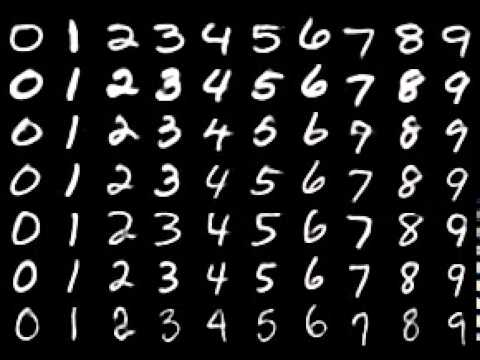
\includegraphics[width=0.4\linewidth]{fig/mnist.jpeg}
\end{center}
\caption{MNIST dataset.}
\vspace*{-3pt}
%{\hfill\footnotesize Note how the caption is centered in the column.\hfill}
\end{figure}

\begin{table}[b]
\begin{center}
\begin{threeparttable}
\caption{Results of experiments conducted by Dahiya et al.}
\begin{tabular}{|c|c|c|r|} \hline
training data & method & SVM kernel& accuracy(\%) \\ \hline\hline
60,000 & Original & - & 97.62 \\ \hline
20,000 & Suport vector & RBF & 97.66 \\ \hline
10,000 & Suport vector & Polynomial & 97.48 \\ \hline
20,000 & Random & - & 95.32 \\ \hline
10,000 & Random & - & 94.67 \\ \hline
\end{tabular}
%\begin{tablenotes}
%\item[a] Uppercase
%\end{tablenotes}
\end{threeparttable}
\end{center}
\end{table}



\section{Training data reduction in deep learning}
In this section, we describe the reduction of training data for deep learning using support vectors. As mentioned in Section 2, since deep learning requires a large amount of training data and learning time, we aim to reduce training data by extracting training data efficiently using support vectors and excluding relatively less critical data. 

\subsection{Training data reduction using support vectors}
This method reduces training data using support vectors to reduce the learning time of the neural network. Fig. 14 shows the proposed method and the learning of a conventional neural network. The procedure of the training data reduction method using support vectors is as follows. 
\begin{enumerate}
\item Train dataset $D$ with SVM and extract support vector $D_{SV}$
\item Train neural networks using $D_{SV}$ as training data
\end{enumerate}
An example of applying data reduction by support vectors to two-dimensional data is shown in Fig. 15. Focus on the following points when using support vectors.
\begin{itemize}
\item How much training data could be reduced
\item How much learning time decreased
\item What is the impact on classification accuracy
\item What happens if the same number of data is randomly extracted for the above three items
\end{itemize}
When using support vectors, if the training data is only slightly reduced, it will be meaningless. It is even more meaningless if degradation in classification accuracy occurs that does not meet the reduction in training data. Also, even if training data can be significantly reduced, classification accuracy must be maintained at a certain level. we will consider the reduction of training data while focusing on these points. However, even if we clear these conditions and confirme that only the support vectors are extracted to reduce the training data and the accuracy hardly falls, this is the undesirable result because there is no meaning using support vectors if the result is almost the same as when data reduction is performed by extracting data at random. It should be kept in mind that this may well occur if the problem to be dealt with is simple, or the training data given originally is excessive. Also, if the classification accuracy is not maintained and degraded when the support vector is used, we consider reinforcing the training data by supplementing the data not extracted as the support vector, as shown in Fig. 15(c). Since part of the data that forms the original space is supplemented, accuracy can be expected to be improved compared to when the training data is only the support vector. 
\begin{figure}[t]
  \begin{center}
  \subfigure[Reduction of training data of neural network using support vector]{
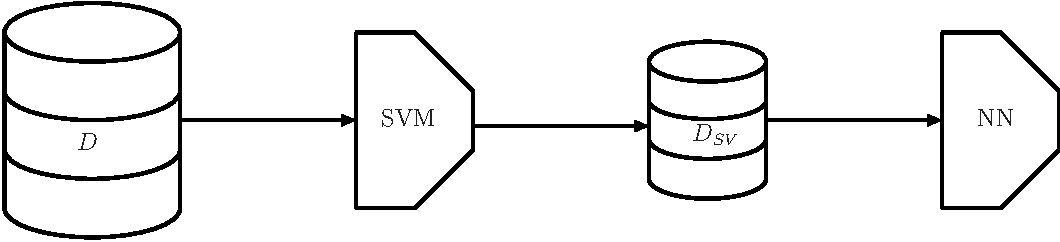
\includegraphics[width=0.8\linewidth]{fig/overview.pdf}}
\subfigure[Normal neural network learning]{
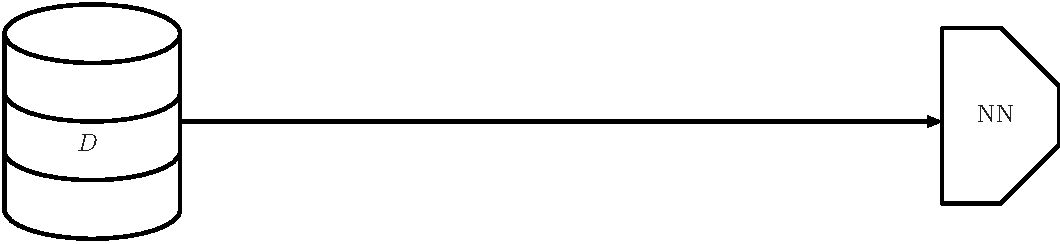
\includegraphics[width=0.8\linewidth]{fig/overview2.pdf}}
\end{center}
\caption{Reduction of training data by support vector.}
\vspace*{-3pt}
%{\hfill\footnotesize Note how the caption is centered in the column.\hfill}
\end{figure}

\begin{figure}[t]
\begin{center}
\subfigure[original data]{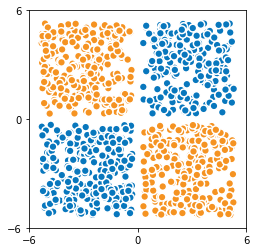
\includegraphics[width=0.3\linewidth]{data/C_XOR/inputdata2.png}}
\subfigure[support vector]{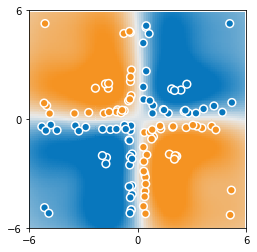
\includegraphics[width=0.3\linewidth]{data/C_XOR/SVMdata2.png}}
\subfigure[support vector + random]{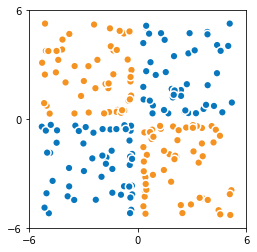
\includegraphics[width=0.3\linewidth]{data/C_XOR/SVM+randomdata.png}}
\end{center}
\caption{Data reduction by support vector and increase of support vector by random sampling data.}
\vspace*{-3pt}
%{\hfill\footnotesize Note how the caption is centered in the column.\hfill}
\end{figure}


\subsection{Preliminary experiment}
In order to confirm the effectiveness of the training data reduction method using support vectors, we evaluate using a program with the same function as TensorFlow Playground\footnote{https://playground.tensorflow.org/} as a preliminary experiment. In the program used, two-dimensional data can be learned with a neural network, and the activation function, the number of intermediate layers, and the number of neurons can be changed arbitrarily. The two-dimensional data used in the evaluation are Gaussian (R\_GAUSS) and straight (R\_PLANE) as two types of regression problems, and Gaussian (C\_GAUSS), spiral (C\_SPIRAL), circle (C\_CIRCLE), and XOR (C\_XOR) as four types of classification problems. We evaluate the amount of data reduction and accuracy and analyze the classification results visually. In the evaluation, we used ReLU as the activation function. The middle layer is three layers, and the number of neurons in each layer is five. When we tried to reduce the data using support vectors for six types of two-dimensional data, almost no deterioration in accuracy occurred in all six. Detailed results are described in Section 4. 

In the preliminary experiment, we evaluate the classification accuracy, regression accuracy, and learning time using training data extracted by the following three methods. 
\begin{enumerate}
\item Learning using all training data
\item Learning using only support vectors
\item Learning extracting randomly as many data as support vectors
\end{enumerate}
The number of epochs is set to 100. However, because C\_SPIRAL is more complicated than the other functions and it takes time, it is set to 500 epochs. Classification accuracy is evaluated by loss, and the smaller the loss, the higher the accuracy. 

\begin{table}[b]
\begin{center}
\begin{threeparttable}
\caption{Type size for papers}
\begin{tabular}{|c|c|c|c|c|c|c|} \hline
\multirow{2}{*}{dataset} & \multicolumn{2}{|c}{(A) All training data} & \multicolumn{2}{|c}{(B) Support vector} & \multicolumn{2}{|c|}{(C)  Random} \\ \cline{2-7}

 & data & loss & data & loss & data & loss \\ \hline\hline
C\_GAUSS & 1,000 & 0.001 & 126 & 0.001 & 126 & 0.001 \\ \hline
R\_PLANE & 2,400 & 0.004 & 292 & 0.001 & 292 & 0.006 \\ \hline
R\_GAUSS & 2,400 & 0.192 & 263 & 0.011 & 263 & 0.563 \\ \hline
C\_SPIRAL & 1,000 & 0.009 & 137 & 0.039 & 137 & 0.105 \\ \hline
C\_CIRCLE & 1,000 & 0.001 & 129 & 0.002 & 129 & 0.177 \\ \hline
C\_XOR & 1,000 & 0.003 & 117 & 0.001 & 117 & 0.005 \\ \hline
\end{tabular}
%\begin{tablenotes}
%\item[a] Uppercase
%\end{tablenotes}
\end{threeparttable}
\end{center}
\end{table}


In C\_GAUSS, the accuracy was not degraded even if learning was performed using only the support vector. However, because the classification is relatively simple, even if it is randomly extracted, the accuracy is hardly degraded, and it can not be determined whether the support vector is capable. As shown in Fig. 16, although it is not classified as a clean straight line like the original data, it can be said that there is no problem because the classification itself is properly performed.

As with C\_GAUSS, R\_PLANE did not degrade in accuracy. Similarly, the effectiveness of the support vector is unknown because accuracy degradation was hardly confirmed even if it was randomly extracted. As can be seen from Fig. 17, it can be said that there is no problem as well as C\_GAUSS because all are classified in the same way.
\begin{figure}[t]
\begin{center}
\subfigure[(A) original data]{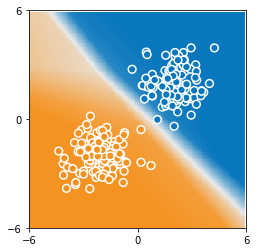
\includegraphics[width=0.40\linewidth]{data/C_GAUSS/result_099.png}}
\subfigure[(B) support vector]{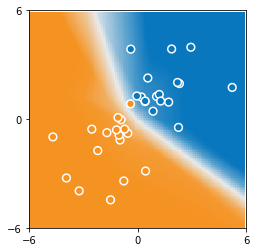
\includegraphics[width=0.40\linewidth]{data/C_GAUSS/SVMresult_099.png}}
\subfigure[(C) random 1]{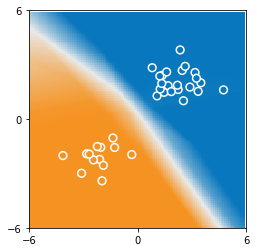
\includegraphics[width=0.40\linewidth]{data/C_GAUSS/Extractedresult_0.png}}
\subfigure[(C) random 2]{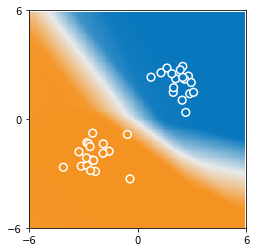
\includegraphics[width=0.40\linewidth]{data/C_GAUSS/Extractedresult_1.png}}
\end{center}
\caption{Evaluation in the dataset C\_GAUSS.}
\vspace*{-3pt}
%{\hfill\footnotesize Note how the caption is centered in the column.\hfill}
\end{figure}

\begin{figure}[t]
\begin{center}
\subfigure[(A) original data]{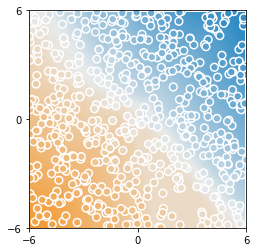
\includegraphics[width=0.40\linewidth]{data/R_PLANE/result_099.png}}
\subfigure[(B) support vector]{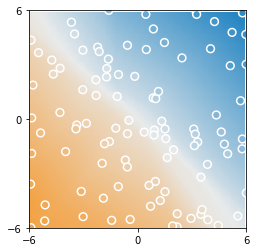
\includegraphics[width=0.40\linewidth]{data/R_PLANE/SVMresult_099.png}}
\subfigure[(C) random 1]{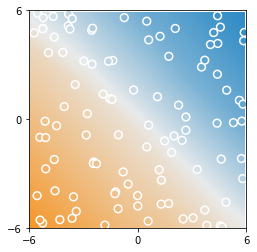
\includegraphics[width=0.40\linewidth]{data/R_PLANE/Extractedresult_0.png}}
\subfigure[(C) random 2]{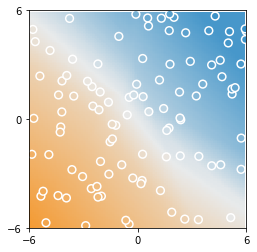
\includegraphics[width=0.40\linewidth]{data/R_PLANE/Extractedresult_3.png}}
\end{center}
\caption{Evaluation in the dataset R\_PLANE.}
\vspace*{-3pt}
%{\hfill\footnotesize Note how the caption is centered in the column.\hfill}
\end{figure}
R\_GAUSS did not lose accuracy even if learning was performed using support vectors only. Besides, the accuracy was degraded in random extraction, and some did not learn well. In R\_GAUSS, a relatively complex data set, the effectiveness of the support vector was shown. Looking at Fig. 18, the support vector can be classified in the same way as the original data, so there is no problem. Also, in some cases, random classification may cause inappropriate classification.

In C\_SPIRAL, although a slight deterioration in accuracy was observed, it was not fatal and was within an acceptable range. Moreover, even if it was extracted at random, there was no significant degradation in accuracy, and it is not clear that the support vector was capable. It can be said that there is no problem because all are classified in the same way, as shown in Fig.19.
\begin{figure}[t]
\begin{center}
\subfigure[(A) original data]{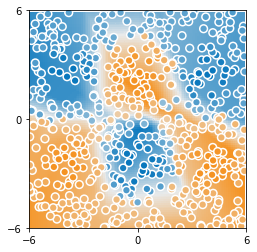
\includegraphics[width=0.40\linewidth]{data/R_GAUSS/result_099.png}}
\subfigure[(B) support vector]{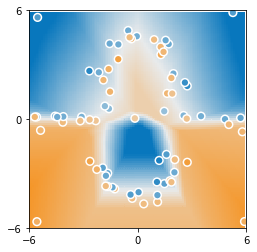
\includegraphics[width=0.40\linewidth]{data/R_GAUSS/SVMresult_099.png}}
\subfigure[(C) random 1]{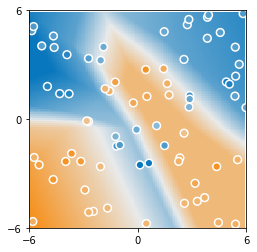
\includegraphics[width=0.40\linewidth]{data/R_GAUSS/Extractedresult_0.png}}
\subfigure[(C) random 2]{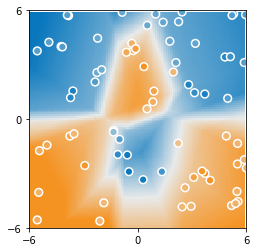
\includegraphics[width=0.40\linewidth]{data/R_GAUSS/Extractedresult_3.png}}
\end{center}
\caption{Evaluation in the dataset R\_GAUSS.}
\vspace*{-3pt}
%{\hfill\footnotesize Note how the caption is centered in the column.\hfill}
\end{figure}
\begin{figure}[t]
\begin{center}
\subfigure[(A) original data]{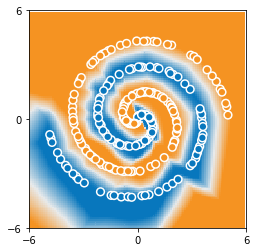
\includegraphics[width=0.40\linewidth]{data/C_SPIRAL/result_499.png}}
\subfigure[(B) support vector]{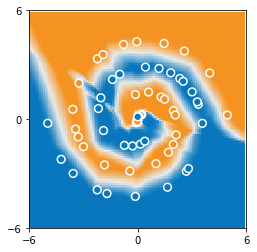
\includegraphics[width=0.40\linewidth]{data/C_SPIRAL/SVMresult_499.png}}
\subfigure[(C) random 1]{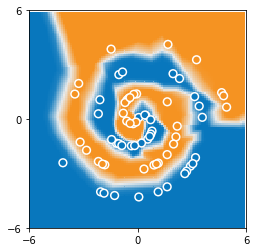
\includegraphics[width=0.40\linewidth]{data/C_SPIRAL/Extractedresult_0.png}}
\subfigure[(C) random 2]{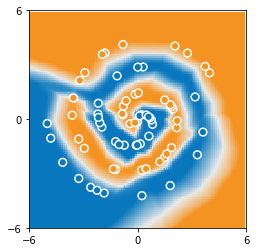
\includegraphics[width=0.40\linewidth]{data/C_SPIRAL/Extractedresult_5.png}}
\end{center}
\caption{Evaluation in the dataset C\_SPIRAL.}
\vspace*{-3pt}
%{\hfill\footnotesize Note how the caption is centered in the column.\hfill}
\end{figure}

The accuracy did not deteriorate even if C\_CIRCLE was trained only with support vectors. However, this is also relatively easy to classify, as in C\_GAUSS so even if it is randomly extracted, its accuracy is hardly degraded, and it can not be concluded that the support vector is capable. Looking at Fig. 20, although random classification sometimes resulted in somewhat angular classification, all classifications were performed without problems within the allowable range.

The accuracy did not deteriorate in the C\_XOR. Besides, even if it was randomly extracted, degradation of accuracy could hardly be confirmed, but there was a case that the classification failed considered once. Therefore, it is considered that the support vector was valid to some extent.

\begin{figure}[t]
\begin{center}
\subfigure[(A) original data]{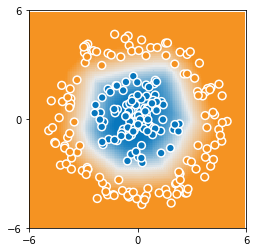
\includegraphics[width=0.40\linewidth]{data/C_CIRCLE/result_099.png}}
\subfigure[(B) support vector]{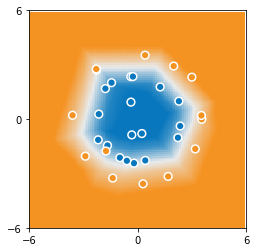
\includegraphics[width=0.40\linewidth]{data/C_CIRCLE/SVMresult_099.png}}
\subfigure[(C) random 1]{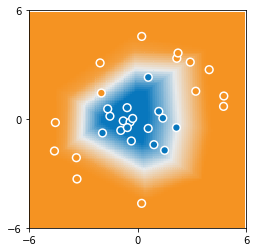
\includegraphics[width=0.40\linewidth]{data/C_CIRCLE/Extractedresult_0.png}}
\subfigure[(C) random 2]{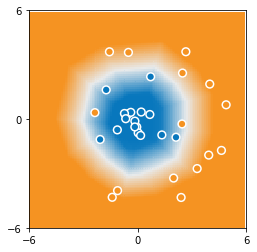
\includegraphics[width=0.40\linewidth]{data/C_CIRCLE/Extractedresult_6.png}}
\end{center}
\caption{Evaluation in the dataset C\_CIRCLE.}
\vspace*{-3pt}
%{\hfill\footnotesize Note how the caption is centered in the column.\hfill}
\end{figure}

\begin{figure}[t]
\begin{center}
\subfigure[(A) original data]{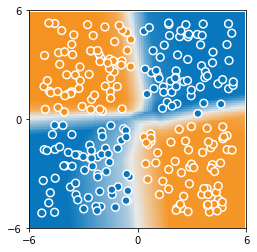
\includegraphics[width=0.40\linewidth]{data/C_XOR/result_099.png}}
\subfigure[(B) support vector]{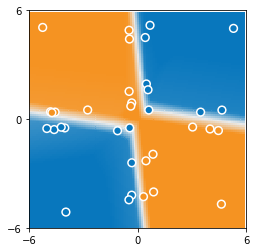
\includegraphics[width=0.40\linewidth]{data/C_XOR/SVMresult_099.png}}
\subfigure[(C) random 1]{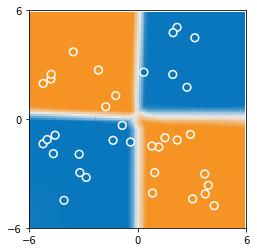
\includegraphics[width=0.40\linewidth]{data/C_XOR/Extractedresult_4.png}}
\subfigure[(C) random 2]{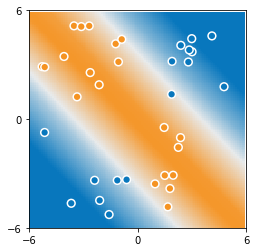
\includegraphics[width=0.40\linewidth]{data/C_XOR/Extractedresult_8.png}}
\end{center}
\caption{Evaluation in the dataset C\_XOR.}
\vspace*{-3pt}
%{\hfill\footnotesize Note how the caption is centered in the column.\hfill}
\end{figure}


%\renewcommand{\textheight}{98mm}

%\newpage
\section{Evaluation}
In this section, the training data reduction method for deep learning with support vectors proposed in Section 3 is applied to ResNet 18 ~\cite{bib:Deep-Residual-Learning-for-Image-Recognition}, which is one of the latest neural networks, and evaluation is performed from the viewpoint of training data reduction and classification accuracy. ResNet is one of the networks achieving high accuracy recognition rate in image recognition. We use the CIFAR-10 ~\cite{bib:Convolutional-Deep-Belief-Networks-on-CIFAR-10} data set for evaluation.
\begin{figure}[t]
\begin{center}
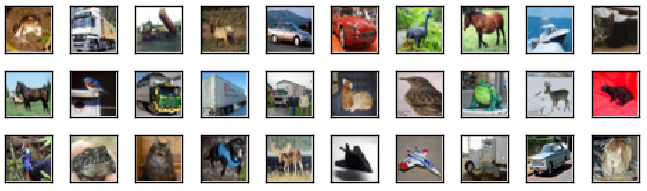
\includegraphics[width=0.95\linewidth]{data/cifar10-2.png}
\end{center}
\caption{A part of CIFAR-10 dataset.}
\vspace*{-3pt}
%{\hfill\footnotesize Note how the caption is centered in the column.\hfill}
\end{figure}

CIFAR-10 is an image data set with a total of 60,000 sheets of 50,000 training data and 10,000 test data.  As shown in Fig. 22, each image is a color image of 3 channels of RGB with $32\times32$ pixels. Each image has a label representing a class, and there are 10 types of class labels: airplane, car, bird, cat, deer, dog, frog, horse, ship, and truck. In this case, two patterns, one for classifying 5 labels, and the other for classifying all 10 labels, are performed. The five labels used for classification are airplanes, birds, deer, frogs and, ships. In all cases, the number of learnings is 100 epochs.

In multiclass classification, since different support vectors are selected for one-to-one classifier and one-to-many classifier, we evaluate both multiclass classification identifications ~\cite{bib:Multi-class-Support-Vector-Machines}. In the one-to-one classifier, ${}_N C _2$ classifiers are used to classify $N$ classes from class $C_1$ to class $C_N$. One-to-many classifiers use N classifiers that solve the two-class classification problem: whether the classification of N classes is classified into a specific class or any other class. 

In the evaluation, we confirme the relationship between classification accuracy and learning time for three cases (A) when using all training data, (B-1) when using only support vectors in a one-to-one classifier and (B-2) when using only support vectors in a one-to-many classifier. Table 3 shows the experimental results for five classes. Table 3 shows that the proposed method reduces the calculation time while achieving the same classification accuracy as the previous method using all the training data. For example, focusing on the calculation accuracy, the calculation accuracy of (A) is 78.300\%, while the calculation accuracy of (B-1) is 78.580\% and (B-2) is 78.340\%, respectively. As for the calculation time, (A) requires 1058.243 seconds for learning, while (B-1) require 961.395 seconds and (B-2) requires 957.629 seconds. In other words, using only the support vector reduced the calculation time by 9.16\% ($1-961.365\div1058.243$) in (B-1) and by 9.50\% ($1-957.629\div1058.243$) in (B-2). Table 4 shows the experimental results for 10 classes. Similar to the evaluation for five classes, the proposed method reduced the calculation time while maintaining the same calculation accuracy as the conventional method. According to Table 4, the calculation time was reduced by 2.54\% ($1-2062.906\div2116.688$) in (B-1) and by 2.66\% ($1-2060.405\div2116.688$) in (B-2). From the above, we confirmed experimentally that the proposed method can reduce the amount of calculation without degradation in accuracy in both 5 label and 10 label evaluations.

It can be read that the reduction effect of calculation time at 10 labels is lower than the effect at 5 labels comparing Table 3 and Table 4. The proposed method reduces the number of data required for training by using only supporter vectors, which is considered to contribute to the reduction of execution results. Focusing on the number of training data required by the conventional method, (B-1) and (B-2), according to Table 3, the number of data is reduced by 11.86\% ($1-22,035\div25,000$) in (B-1) and 12\% ($1-21,975\div25,000$) in (B-2) at 5 labels, respectively. Similarly, according to Table 4, the reduction rate of the number of training data at 10 labels is 4.26\% ($1-47,870\div50,000$) and 4.40\% ($1-47,799\div50,000$). Similar to the reduction rate of calculation time, it can be read that the reduction rate of the number of training data at 5 labels is higher than at 10 labels. 

Based on the above experimental results, we consider training data reduction when using support vectors for CIFAR-10. The preliminary experiments in Section 3.2 reduced the original data by 86 to 88\% when determining the support vector. However, when the support vector was extracted from the training data of CIFAR-10, it was only reduced by about 12\% of the original data in the case of 5 labels. It accounted for a large proportion of the original data and did not provide the expected results from the preliminary experiments in terms of reduction of training data. The cause of this problem is that the problem of identifying color images is much more complicated than that of the preliminary experiments. In the case of a relatively simple data set as treated in the preliminary experiment, no deterioration in accuracy was observed even if the number of data extracted as support vectors was 12 to 14\%. However, in the case of relatively complex data sets such as CIFAR-10, as there are many data responsible for the formation of the classification plane, the number of training data extracted as support vectors is about 88\%, which is the majority of the whole. Compared with the results of the preliminary experiments, although it did not reduce the training data as expected, the training data could be reliably reduced. Moreover, since the accuracy has hardly been deteriorated, it is possible to improve the trade-off between the number of training data and the classification accuracy and to reduce the training data of CIFAR-10 without causing the accuracy deterioration by using the support vector. Compared with the results of the random sampling data performed as a control experiment, the accuracy is also improved, although it is about 1\%. Also, the time taken for learning decreased with the reduction of training data, and it can be said that this was also effective. There were more data extracted as support vectors for 10 labels than for 5 labels, and about 95\% was extracted. Although only 5\%, this was also able to reduce training data. As in the case of 5 labels, almost no degradation in accuracy occurs, so it can be said that the effect of the support vector has been confirmed.

\begin{table}[b]
\begin{center}
\begin{threeparttable}
\caption{Result of applying support vector for CIFAR-10 (5 labels)}
\begin{tabular}{|l|r|c|r|} \hline
training data & data & accuracy(\%) & time(sec) \\ \hline\hline
(A) all data & 25,000 & 78.300 &1058.243 \\ \hline
(B-1) support vector(one-to-one) & 22,035 & 78.580 & 961.394 \\ \hline
(B-2) support vector(one-to-many) & 21,975 & 78.340 & 957.629 \\ \hline
(C-1) random & 22,035 & 77.400 & 962.348 \\ \hline
(C-2) random & 21,975 & 77.260 & 959.526 \\ \hline
\end{tabular}
%\begin{tablenotes}
%\item[a] Uppercase
%\end{tablenotes}
\end{threeparttable}
\end{center}
\end{table}

\begin{table}[b]
\begin{center}
\begin{threeparttable}
\caption{Result of applying support vector for CIFAR-10 (5 labels)}
\begin{tabular}{|l|r|c|r|} \hline
training data & data & accuracy(\%) & time(sec) \\ \hline\hline
(A) all data & 50,000 & 77.560 & 2116.688 \\ \hline
(B-1) support vector(one-to-one) & 47,870 & 77.420 & 2062.906 \\ \hline
(B-2) support vector(one-to-many) & 47,799 & 76.970 & 2060.405 \\ \hline
(C-1) random & 47,870 & 76.580 & 2052.179 \\ \hline
(C-2) random & 47,799 & 76.290 & 2057.681 \\ \hline
\end{tabular}
%\begin{tablenotes}
%\item[a] Uppercase
%\end{tablenotes}
\end{threeparttable}
\end{center}
\end{table}






\section{Conclusions}
In this study, we tried to reduce training data in deep learning by using support vectors. Although several existing studies used data reduction by support vectors, the difference from them is that support vectors are applied to CIFAR-10. First, we conducted preliminary experiments to reduce training data using support vectors for six types of two-dimensional data, and it was confirmed that training data could be reduced by 86 to 88\% while maintaining the accuracy. Based on this, when trying to reduce training data using support vectors for the problem of classifying CIFAR-10 color images as well, The training data could be reduced by about 12\% in the 5-class classification and about 5\% in the 10-class classification with almost no deterioration in accuracy. Although the effect was not obtained like the result of the experiment, it was confirmed that the training data could be reduced by using the support vector for CIFAR-10 as well.

\section*{Acknowledgment}

\bibliographystyle{IEEEtran}
\bibliography{IEEEfull,full,refs}

%\begin{thebibliography}{1}

%\bibitem{1}
\if0
G.~Eason, B.~Noble, and I.~N.~Sneddon, ``On certain integrals of
Lipschitz-Hankel type involving products of Bessel functions,''
\emph{Phil. Trans. Roy. Soc. London,} vol. A247, pp. 529-551, April
1955.

\bibitem{2}
J.~Clerk~Maxwell, \emph{A Treatise on Electricity and Magnetism,}
3$^{\rm rd}$ ed., vol. 2. Oxford: Clarendon, 1892, pp.68-73.

\bibitem{3}
I.~S.~Jacobs and C.~P.~Bean, ``Fine particles, thin films and exchange
anisotropy,'' in \emph{Magnetism,} vol. III, G.T. Rado and H. Suhl,
Eds. New York: Academic, 1963, pp. 271-350.

\bibitem{4}
K.~Elissa, ``Title of paper if known,'' unpublished.

\bibitem{5}
R.~Nicole, ``Title of paper with only first word capitalized,''
\emph{J. Name Stand. Abbrev.,} in press.

\bibitem{6}
Y.~Yorozu, M.~Hirano, K.~Oka, and Y.~Tagawa, ``Electron spectroscopy
studies on magneto-optical media and plastic substrate interface,''
\emph{APSIPA Transl. J. Magn. Japan,} vol. 2, pp. 740-741, August 1987
[\emph{Digests 9$^{\rm th}$ Annual Conf. Magnetics Japan,} p. 301,
1982].

\bibitem{7}
M.~Young, \emph{The Technical Writer's Handbook.} Mill Valley, CA:
University Science, 1989.
\fi
%\end{thebibliography}
\end{document}
